\chapter{Cortafuegos: Casos de estudio}
\section{\it Firewall-1}
\subsection{Introducci\'on}
Quiz\'as el cortafuegos m\'as utilizado actualmente en Internet es {\it 
FireWall-1}, desarrollado por la empresa israel\'{\i} {\it Check Point Software 
Technologies Ltd.} ({\tt http://www.checkpoint.com/}). Este {\it firewall} se
ejecuta sobre diferentes sistemas Unix (Solaris, AIX, Linux y HP-UX), as\'{\i}
como sobre Windows NT y tambi\'en en `cajas negras' como las desarrolladas
por Nokia, que poseen un sistema operativo propio (IPSO) basado en FreeBSD.\\
\\Quiz\'as la caracter\'{\i}stica m\'as importante de {\it Firewall-1} sea que
incorpora una nueva arquitectura dentro del mundo de los cortafuegos: la 
inspecci\'on con estado ({\it stateful inspection}). {\it Firewall-1} inserta 
un m\'odulo denominado {\it Inspection Module} en el n\'ucleo del sistema 
operativo sobre el que se instala, en el nivel {\it software} m\'as bajo 
posible (por debajo incluso del nivel de red), tal y como se muestra en la 
figura \ref{fw1}; as\'{\i}, desde ese nivel tan bajo, {\it Firewall-1} puede 
interceptar y analizar todos los paquetes antes de que lleguen al resto del 
sistema: se garantiza que ning\'un paquete es procesado por ninguno de los 
protocolos superiores hasta que {\it Firewall-1} comprueba que no viola la 
pol\'{\i}tica de seguridad definida en el cortafuegos.\\
\begin{figure}
\begin{center}
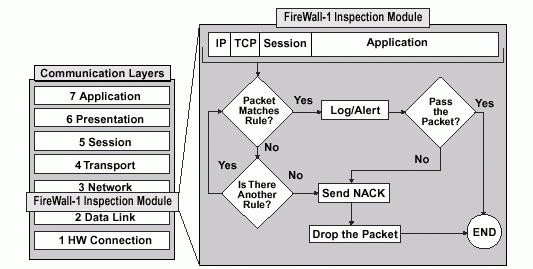
\includegraphics[width=\textwidth]{fw1.png}
\caption{Ubicaci\'on del {\it Inspection Module} dentro de la pila de 
protocolos {\sc osi}.}
\label{fw1}
\end{center}
\end{figure}
\\{\it Firewall-1} es capaz de analizar la informaci\'on de una trama en cada
uno de los siete niveles OSI y a la vez analizar informaci\'on de estado 
registrada de anteriores comunicaciones; el cortafuegos entiende la estructura
de los diferentes protocolos {\sc tcp/ip} -- incluso de los ubicados en la
capa de aplicaci\'on --, de forma que el {\it Inspection Module} extrae 
la informaci\'on relevante de cada paquete para construir tablas din\'amicas
que se actualizan constantemente, tablas que el {\it firewall} utiliza para
analizar comunicaciones posteriores. En el m\'odulo de inspecci\'on se 
implantan las pol\'{\i}ticas de seguridad definidas en cada organizaci\'on
mediante un sencillo lenguaje denominado {\sc inspect}, tambi\'en dise\~nado
por {\it Check Point Software Technologies}; desde un c\'omodo interfaz se 
genera un {\it script} en este lenguaje, que se compila y se inserta en el {\it 
Inspection Module}.\\
\\La gran potencia y flexibilidad de {\it Firewall-1} hacen imposible que se
aqu\'{\i} se puedan explicar con el suficiente nivel de detalle todas sus 
caracter\'{\i}sticas; para m\'as informaci\'on, excelentes lecturas pueden ser 
\cite{kn:gon99} o (m\'as reciente) \cite{kn:phone02}. Tambi\'en la 
documentaci\'on que acompa\~na al producto, y la disponible en el servidor
{\it web} de {\it Check Point Software Technologies}, es de gran ayuda para
cualquier administrador que utilice este cortafuegos en su red.
\subsection{Arquitectura}
{\it Firewall-1} est\'a basado en dos m\'odulos independientes: el de gesti\'on
(o control)
y el de cortafuegos. El primero de ellos est\'a formado por el gestor gr\'afico
de pol\'{\i}ticas (incluyendo el visor de registros) y el servidor de gesti\'on,
t\'{\i}picamente un demonio ({\tt fwm}) que se ejecuta en una m\'aquina Unix. El
gestor gr\'afico puede ser un cliente Unix (con X/Motif) o Windows 9x/NT; es
triste que a estas alturas no exista un cliente gr\'afico para Linux, 
encontr\'andose \'unicamente para otros Unices, y que adem\'as el cliente 
X/Motif contenga errores y sea bastante ineficiente, lo que motiva que se 
tienda a utilizar clientes Windows para gestionar los cortafuegos. En cualquier 
caso, el gestor gr\'afico puede ejecutarse en la misma m\'aquina que el 
servidor de gesti\'on o en una diferente, mediante un esquema cliente/servidor. 
Este gestor no hace m\'as que presentar de una forma c\'omoda al administrador 
del cortafuegos la informaci\'on generada por el servidor de gesti\'on (el 
demonio {\tt fwm}), que es el verdadero `coraz\'on' de la gesti\'on del {\it 
firewall} y que permite administrar diferentes sistemas con m\'odulo de 
cortafuegos (en castellano plano, diferentes cortafuegos) desde una misma 
estaci\'on de control.\\
\\Por otra parte, el m\'odulo de cortafuegos est\'a formado por el {\it 
inspection module}, los demonios de {\it Firewall-1} y los servidores de 
seguridad del {\it firewall}. El {\it inspection module} se instala como ya
hemos comentado (figura \ref{fw1}) entre el nivel de enlace y el nivel de red, 
por completo antes de la pila de protocolos {\sc tcp/ip}, con lo que se asegura
que {\it Firewall-1} analiza todos y cada uno de los paquetes que pasan por el
sistema. Los demonios del {\it firewall} son simples programas con diferentes
funciones, como la comunicaci\'on con el servidor de gesti\'on o la carga de las
reglas definidas para el cortafuegos en el {\it inspection module}. Finalmente, 
los servidores de seguridad son m\'odulos que se invocan cuando 
as\'{\i} se define en la pol\'{\i}tica (por ejemplo, cuando la acci\'on asociada
a una determinada regla es {\tt User Authentication}), y que realizan tareas
de autenticaci\'on y seguridad de contenidos; la conexi\'on entre origen y 
destino se divide en dos, una entre el origen y el servidor de seguridad y otra
entre este y el destino.
\subsection{Instalaci\'on}
Antes de instalar {\it Firewall-1} en un sistema Unix es {\bf muy importante} 
deshabilitar en el n\'ucleo del operativo el {\it IP Forwarding}, de forma que
todo el reenv\'{\i}o de tramas sea gestionado por el {\it software} de
cortafuegos (esta opci\'on se define durante la instalaci\'on). Esto permite 
que el reenv\'{\i}o s\'olo sea posible si el {\it
firewall} est\'a ejecut\'andose -- es decir, protegiendo nuestra red --, lo que
imposibilita que la m\'aquina reenv\'{\i}e paquetes si {\it Firewall-1} no
est\'a activo, algo que como vimos a la hora de hablar de diferentes clones de
Unix puede ser problem\'atico para nuestra seguridad.\\
\\Teniendo en cuenta la consideraci\'on anterior, y asumiendo que en la 
m\'aquina donde vamos a instalar {\it Firewall-1} no existen problemas ajenos
al cortafuegos (conectividad, resoluci\'on de nombres, reconocimiento de 
interfaces de red\ldots), la instalaci\'on del {\it software} no ofrece ninguna 
dificultad: simplemente hemos de instalar los paquetes correspondientes con las 
\'ordenes habituales de cada Unix ({\tt pkgadd} en Solaris, {\tt swinstall} en
HP-UX\ldots) o, en algunas versiones del programa, ejecutar la orden {\tt 
fwinstall}, que no es m\'as que una instalaci\'on seguida de una 
configuraci\'on del cortafuegos equivalente a la que veremos a continuaci\'on.\\
\\Una vez instalado el {\it firewall} hemos de configurarlo; para ello no 
tenemos m\'as que ejecutar la orden {\tt fwconfig} (versi\'on 4.0) o {\tt 
cpconfig} (versi\'on 4.1), que paso a paso nos guiar\'a a trav\'es de la 
configuraci\'on (o reconfiguraci\'on, una vez el cortafuegos est\'e ya
funcionando) de {\it Firewall-1}: 
\begin{quote}
\begin{verbatim}
anita:/# fwconfig

Welcome to VPN-1 & FireWall-1 Configuration Program
=================================================
This program will let you re-configure
your VPN-1 & FireWall-1 configuration.


Configuration Options:
----------------------
(1)  Licenses
(2)  Administrators
(3)  GUI clients
(4)  Remote Modules
(5)  SMTP Server
(6)  SNMP Extension
(7)  Groups
(8)  IP Forwarding
(9)  Default Filter
(10) CA Keys

(11) Exit

Enter your choice (1-11) : 11

Thank You...
anita:/#
\end{verbatim}
\end{quote}
Como podemos ver, esta herramienta permite realizar tareas como la 
instalaci\'on de licencias, la planificaci\'on del {\it software} en el 
arranque de la m\'aquina o la definici\'on de m\'odulos de {\it firewall} 
remotos. Aunque todo es 
vital para el correcto funcionamiento del cortafuegos, existen dos apartados 
especialmente importantes para la posterior gesti\'on del {\it firewall}: la
definici\'on de administradores y la definici\'on de estaciones que actuar\'an 
como clientes gr\'aficos; si no definimos al menos un administrador y una
estaci\'on cliente, no podremos acceder al cortafuegos para gestionarlo 
(evidentemente, en esta situaci\'on no estar\'{\i}a todo perdido, ya que siempre
podemos a\~nadir ambos elementos, as\'{\i} como modificar su relaci\'on, {\it a 
posteriori}).\\
\\El administrador o administradores que definamos ser\'an los encargados de 
acceder a las pol\'{\i}ticas del cortafuegos a trav\'es del gestor gr\'afico, 
\'unicamente desde las estaciones que hayamos definido como cliente. Podemos
a\~nadir elementos a ambas listas (la de administradores y la de estaciones 
gr\'aficas) ejecutando de nuevo {\tt fwconfig} o {\tt cpconfig}, o bien de forma
m\'as directa ejecutando la orden {\tt fwm} (para a\~nadir administradores) y
modificando el archivo {\tt \$FWDIR/conf/gui-clients} (para a\~nadir clientes
gr\'aficos); este archivo no es m\'as que un fichero de texto donde se listan
las direcciones IP (o los nombres DNS) de las m\'aquinas que pueden acceder
a gestionar el {\it firewall}:
\begin{quote}
\begin{verbatim}
anita:/# cat $FWDIR/conf/gui-clients
192.168.0.1
192.168.0.2
192.168.0.3
158.42.22.41
anita:/# fwm -p
FireWall-1 Remote Manager Users:
================================
toni (Read/Write)
avh (Read/Write)

Total of 2 users
anita:/# fwm -a admin -wr
Password:
Verify Password:
User admin added succesfully
anita:/# fwm -p
FireWall-1 Remote Manager Users:
================================
toni (Read/Write)
avh (Read/Write)
admin (Read Only)

Total of 3 users
anita:/# fwm -r prova
User prova removed succesfully
anita:/#
\end{verbatim}
\end{quote}
Para acabar con la instalaci\'on de {\it Firewall-1} es necesario definir la
variable de entorno {\tt \$FWDIR}, que apuntar\'a al directorio {\tt /etc/fw/},
y a\~nadirla en los {\it scripts} de inicio de sesi\'on correspondientes. 
Tambi\'en es recomendable a\~nadir el directorio {\tt \$FWDIR/bin/} a nuestro
{\it \$PATH}, ya que ah\'{\i} se ubican las utilidades de gesti\'on del
cortafuegos, y hacer lo mismo con {\tt \$FWDIR/man/} y la variable {\it 
\$MANPATH}, ya que en este directorio se encuentran las p\'aginas de manual del
{\it firewall}.\\
\\Antes de finalizar este punto quiz\'as es necesaria una peque\~na 
advertencia: como {\it Firewall-1} inserta
m\'odulos en el n\'ucleo del operativo, es dependiente de la versi\'on del
{\it kernel} utilizada. Todas las versiones m\'as o menos modernas funcionan
correctamente sobre Solaris 2.6 y la \'ultima tambi\'en sobre Solaris 7; no 
obstante, sobre este \'ultimo el resto de versiones no funcionan bien, aunque
se instalen correctamente. Es posible, y esto lo digo por experiencia, que la
m\'aquina no arranque tras instalar el {\it software} debido a las 
modificaciones de los {\it scripts} de arranque (concretamente los ubicados en
{\tt /etc/rcS.d/}), que al ser invocados desde {\tt /sbin/rcS} producen errores
que impiden montar correctamente los discos y proseguir el arranque; para 
solucionar estos problemas, lo m\'as r\'apido es eliminar cualquier 
modificaci\'on que la instalaci\'on de {\it Firewall-1} haya realizado sobre
los programas ejecutados al iniciar el sistema. 
\subsection{Gesti\'on}
Como cualquier sistema cortafuegos, {\it Firewall-1} permite al usuario definir
una pol\'{\i}tica de seguridad formada por reglas, cada una de las cuales se 
basa principalmente en el origen, destino y servicio de una determinada trama. 
El conjunto de reglas se examina de arriba hacia abajo, de forma que si una 
determinada regla hace {\it match} con el paquete que se est\'a inspeccionando,
se aplica y las que quedan por debajo de ella ni siquiera se examinan; como
deber\'{\i}a suceder en cualquier sistema cortafuegos, las tramas no 
expl\'{\i}citamente aceptadas se rechazan.\\
\\La gesti\'on de {\it Firewall-1} suele ser completamente gr\'afica, a trav\'es
de dos interfaces principales: el de gesti\'on de pol\'{\i}ticas ({\tt fwui}) y 
el visor de {\it logs} ({\tt fwlv}, mostrado en la figura \ref{fwlv}). En 
versiones m\'as recientes del {\it firewall} ambos se unifican en {\tt 
fwpolicy}, basado en X/Motif (los anteriores se basan en OpenLook), m\'as 
c\'omodo e intuitivo que sus predecesores. En cualquier caso, siempre tenemos la
opci\'on de trabajar en modo texto mediante la orden {\tt fw}, aunque esta
opci\'on no suele ser la habitual entre los administradores de {\it 
Firewall-1}.\\
\\Para gestionar el cortafuegos, cada uno de los administradores definidos 
anteriormente puede conectar desde las estaciones gr\'aficas autorizadas al 
servidor de gesti\'on (m\'aquina en la que se ha instalado el m\'odulo de 
gesti\'on de {\it Firewall-1}), para lo cual necesita autenticarse mediante su 
nombre de usuario y su clave; una vez conectado, si su acceso es de lectura y 
escritura, puede comenzar a trabajar con el cortafuegos. Lo primero que ver\'a 
ser\'a la pol\'{\i}tica del {\it firewall} (de hecho, ha conectado con el 
editor de pol\'{\i}ticas de {\it Firewall-1}); estas pol\'{\i}ticas no son m\'as
que ficheros ubicados en {\tt \$FWDIR/conf/}, con un nombre finalizado en {\tt
`.W'}, que se compilan y cargan en los sistemas donde est\'a instalado el 
m\'odulo de cortafuegos.\\
\\Desde el editor gr\'afico, las pol\'{\i}ticas se ven como un conjunto de 
reglas que se examina de arriba a abajo hasta que una de ellas hace {\it match}
con el paquete que se est\'a analizando (como ya hemos comentado, si ninguna de
ellas hace {\it match}, el paquete se deniega). Cada una de estas reglas est\'a
numerada en funci\'on del orden de aplicaci\'on, y sus campos principales son 
los habituales en cualquier cortafuegos: origen, destino, servicio y acci\'on.
Adem\'as, existen un campo que indica si se ha de registrar la trama ({\tt 
`Track'}), otro para determinar d\'onde se ha de instalar ({\tt `Install On'}), 
otro para especificar el tiempo que la regla estar\'a activa ({\tt `Time'}) y
finalmente un campo de texto donde se pueden incluir comentarios.\\
\\Evidentemente, como sucede en cualquier {\it firewall}, tanto el campo origen 
como el destino pueden ser sistemas concretos o redes completas. En {\it 
Firewall-1} ambos elementos, as\'{\i} como los servicios, se manejan como {\bf 
objetos}: elementos definidos por el administrador e identificados mediante un
nombre -- en principio algo f\'acilmente identificable por el mismo --, con una
serie de propiedades determinadas. Sin duda, en el caso de los {\it hosts} o las
redes la propiedad m\'as importante es la direcci\'on IP o la direcci\'on de 
red con su m\'ascara correspondiente asociadas al objeto; en el caso de los
servicios, definidos tambi\'en por un nombre, la caracter\'{\i}stica m\'as
importante es el puerto o rango de puertos asociado al mismo. Por ejemplo, 
podemos definir el objeto {\it `servidor1'}, con su IP correspondiente, el 
objeto {\it DMZ}, con su direcci\'on de red y m\'ascara asociada, o el objeto
{\it ssh}, con su puerto concreto; en todos los casos, el nombre dice mucho 
m\'as al encargado de gestionar el cortafuegos que una simple IP, direcci\'on 
de red o n\'umero de puerto, lo que facilita enormemente la administraci\'on 
del {\it firewall}.\\
\\El campo {\tt `Action'} de cada regla define qu\'e se ha de hacer con una
conexi\'on cuando hace {\it match} con la regla; al igual que en la mayor parte
de cortafuegos del mercado, tres son las acciones principales a tomar: {\tt
`Accept'}, si dejamos que la conexi\'on se establezca a trav\'es del {\it 
firewall}, {\tt `Reject'}, si la rechazamos, y {\tt `Drop'}, si la rechazamos 
sin notificarlo al origen. Para las conexiones que no permitimos, esta \'ultima
suele ser la mejor opci\'on, ya que el paquete se elimina sin ning\'un tipo de
notificaci\'on hacia el origen; si utiliz\'aramos {\tt `Reject'} s\'{\i} que
informar\'{\i}amos de las conexiones no permitidas, lo que puede ayudar a un
atacante a conocer tanto nuestra pol\'{\i}tica de seguridad como la 
topolog\'{\i}a de nuestra red.\\
\\Por su parte, el campo {\tt `Track'} de una regla determina una medida a 
tomar cuando un paquete hace {\it match} con la regla en cuesti\'on: ninguna
medida (campo vac\'{\i}o), un registro en diferentes formatos ({\tt `Short 
Log'}, {\tt `Long Log'} y {\tt `Accounting'}), una alerta de seguridad, un 
correo electr\'onico, un {\it trap} {\sc snmp} o una acci\'on definida por el
usuario (estas cuatro \'ultimas acciones han de ser configuradas por el 
administrador del cortafuegos). Evidentemente, este campo es muy \'util para 
obtener informaci\'on acerca de posibles hechos que traten de comprometer 
nuestra seguridad, tanto en un {\it log} habitual como para implantar en el {\it
firewall} un sistema de detecci\'on de intrusos y respuesta autom\'atica en
tiempo real (\cite{kn:spi01b}); en el punto \ref{fw1log} hablaremos con m\'as
detalle del sistema de {\it log} de {\it Firewall-1}.\\
\\Una vez que hemos definido una pol\'{\i}tica -- un conjunto de reglas -- lo
m\'as habitual es aplicarla en un sistema con el m\'odulo de cortafuegos de {\it
Firewall-1} instalado en \'el; hemos de recordar que habitualmente trabajamos 
con un simple {\bf editor} de pol\'{\i}ticas, de forma que las modificaciones 
que realicemos sobre una determinada pol\'{\i}tica (a\~nadir o eliminar reglas,
definir nuevos objetos, etc.) no tendr\'an ning\'un efecto hasta que esa 
pol\'{\i}tica se instale en el cortafuegos correspondiente. Para instalar una
pol\'{\i}tica no tenemos m\'as que escoger la opci\'on del men\'u del gestor
gr\'afico adecuada; a partir de ese momento, {\it Firewall-1} verifica que la 
pol\'{\i}tica escogida es l\'ogica y consistente, genera y compila el c\'odigo 
{\sc inspect} (en el punto \ref{inspect} hablamos m\'{\i}nimamente de este
lenguaje) correspondiente para cada objeto sobre el que vayamos a instalarla, y 
carga dicho c\'odigo en el objeto donde se encuentra el m\'odulo de cortafuegos
a trav\'es de un canal seguro.
\begin{figure}
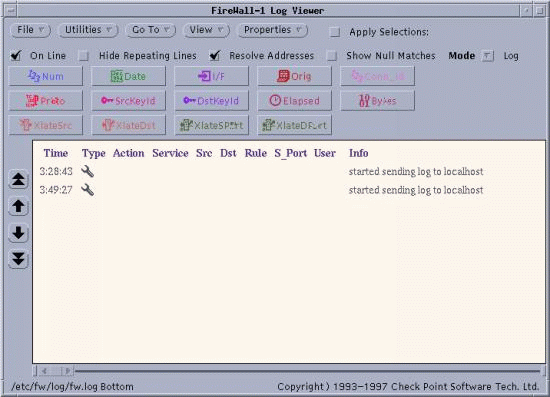
\includegraphics[width=\textwidth]{fwlv.png}
\caption{Una imagen de {\tt fwlv}.}
\label{fwlv}
\end{figure}
\subsection{El sistema de {\it log}}
\label{fw1log}
Cuando una regla tiene definido en el campo {\tt Track} que guarde un {\it log},
siempre que una trama haga {\it match} con la misma se generar\'a un registro
del evento, tanto si la conexi\'on se acepta como si se deniega. A diferencia 
de la mayor parte del {\it software} de un sistema Unix, los {\it 
logs} de {\it Firewall-1} no son simples ficheros ASCII, sino que se almacenan
en un formato propio dentro del directorio {\tt \$FWDIR/logs/}. Para 
consultarlos hemos de utilizar o bien el visor gr\'afico {\tt fwlv} (figura
\ref{fwlv}) o bien la orden {\tt fw}, que tambi\'en permite rotarlos ({\tt `fw
logswitch'}) y exportarlos a ficheros ASCII ({\tt `fw logexport'}):
\begin{quote}
\begin{verbatim}
anita:/etc/fw/bin# ./fw log
Date: May 2, 2000
 3:28:43 ctl    anita      >daemon started sending log to localhost
 3:49:27 ctl    anita      >daemon started sending log to localhost
 4:30:30 ctl    anita      >daemon started sending log to localhost
anita:/etc/fw/bin# ./fw logexport -o /etc/fw/logs/salida.ascii
Starting pass 1 of the log file.
Starting pass 2 of the log file..
   100.00% of log file processed.

anita:/etc/fw/bin# cat /etc/fw/logs/salida.ascii
num;date;time;orig;type;action;alert;i/f_name;i/f_dir;sys_msgs
0;2May2000; 3:28:43;anita;control;ctl;;daemon;inbound;started sending log
to localhost
1;2May2000; 3:49:27;anita;control;ctl;;daemon;inbound;started sending log
to localhost
2;2May2000; 4:30:30;anita;control;ctl;;daemon;inbound;started sending log
to localhost

anita:/etc/fw/bin#
\end{verbatim}
\end{quote}
Evidentemente, rotar los {\it logs} o exportarlos a ficheros ASCII nos puede
resultar muy \'util a la hora de realizar estad\'{\i}sticas o tareas 
similares, ya que podemos
separar los registros por d\'{\i}as, meses, horas\ldots o cualquier otro 
par\'ametro que se nos ocurra y utilizar las herramientas propias de cualquier
Unix ({\tt awk}, {\tt perl}, {\tt grep}\ldots) sobre el fichero de texto para
extraer el tipo de registros que nos interese; no obstante, esto a todas luces
presenta un grave inconveniente: los registros de {\it Firewall-1}, con lo que
hemos visto hasta ahora, no pueden utilizarse para monitorizar el tr\'afico en 
tiempo real o para ofrecer una respuesta autom\'atica ante un ataque. Por
supuesto, la detecci\'on de un ataque {\it offline}, sobre un fichero de
registro hist\'orico (por ejemplo, podemos buscar tr\'afico sospechoso cada 
noche sobre el {\it log} del d\'{\i}a anterior) es muy importante, pero sin
duda lo es m\'as el que seamos capaces de detectar ese mismo ataque justo
cuando se est\'a produciendo, para ofrecer as\'{\i} una respuesta inmediata y
minimizar el riesgo asociado a las actividades de un pirata; cuanto m\'as
tardemos, m\'as posibilidades tiene el atacante de tener \'exito en su tarea
(\cite{kn:coh99}).\\
\\Para implantar un sistema de respuesta autom\'atica en tiempo real, o 
simplemente para visualizar los registros generados por el cortafuegos tambi\'en
en tiempo real podemos utilizar la orden {\tt `fw log'}, que con las opciones
adecuadas imprimir\'a en pantalla cualquier registro que se genere al mismo 
tiempo que la entrada se guarda en el fichero de {\it log} correspondiente con 
el formato propio de {\it Firewall-1}:
\begin{quote}
\begin{verbatim}
anita:/# fw log -f -n |head -3
2:21:12 drop   anita   >nei0 proto tcp src 192.168.0.3 dst 158.42.22.41 \
service finger s_port 13000 len 40 rule 5 
2:22:23 drop   anita   >nei0 proto tcp src 192.168.0.10  dst 158.42.2.1 \
service NetBus s_port 32344 len 40 rule 6 
2:22:45 drop   anita   >nei0 proto tcp src 192.168.0.1  dst 192.168.2.3 \
service echo-tcp s_port 30298 len 40 rule 5
anita:/#
\end{verbatim}
\end{quote}
Como vemos, la salida de esta orden ya puede ser
procesada desde l\'{\i}nea de comandos con las herramientas habituales de Unix
para implantar as\'{\i} la respuesta autom\'atica, por ejemplo mediante {\tt
`fw sam'}, que bloquea todo el tr\'afico proveniente de una determinada 
direcci\'on en el cortafuegos, de forma permanente o temporal 
(\cite{kn:spi01b}). 
\subsection{\sc inspect}
\label{inspect}
Como ya hemos comentado, al instalar una pol\'{\i}tica en un cortafuegos 
(m\'aquina con el m\'odulo de {\it firewall}) desde el servidor de gesti\'on
(m\'aquina donde se ha instalado el {\it Management Module}) {\it Firewall-1} 
genera en el mismo servidor de gesti\'on un c\'odigo -- un {\it script}, un
simple fichero ASCII editable -- en un lenguaje de alto nivel propio de {\it 
Firewall-1}: este lenguaje se denomina {\sc inspect}, es orientado a objetos, y 
est\'a dise\~nado expl\'{\i}citamente 
para trabajar con cortafuegos, lo que permite por ejemplo programar las 
acciones t\'{\i}picas de un {\it firewall}: detener una trama, aceptarla, 
generar un registro\ldots\\ 
\\El {\it script} de {\sc inspect} generado a partir de la pol\'{\i}tica editada
en el gestor gr\'afico (o desde l\'{\i}nea de comandos, mediante la orden {\tt
`fw gen'}) es un fichero {\tt `.pf'} que se encuentra en {\tt
\$FWDIR/conf/}; este archivo es compilado mediante {\tt fwc} y a partir de \'el 
se genera un c\'odigo (un fichero {\tt `.fc'}) dentro de {\tt \$FWDIR/tmp/}
junto a otros archivos adicionales en el mismo directorio. Como hemos dicho el
c\'odigo generado se transmite al m\'odulo 
de cortafuegos a trav\'es de un canal seguro, y en este m\'odulo los demonios de
{\it Firewall-1} son los encargados de cargar el c\'odigo en el n\'ucleo del
operativo, comenzando as\'{\i} a ser operativa la nueva pol\'{\i}tica.\\
\\La carga del c\'odigo en el cortafuegos se realiza de forma autom\'atica tras
generar y compilar el fichero {\tt `.pf'} desde el editor gr\'afico de 
pol\'{\i}ticas, aunque puede llevarse a cabo manualmente mediante \'ordenes como
{\tt `fw load'} o {\tt `fw fetch'}; este c\'odigo se ejecuta en una m\'aquina
virtual ubicada en el n\'ucleo del operativo, y su ejecuci\'on b\'asicamente
consiste en inspeccionar todas las tramas que pasan por el {\it firewall} para
decidir qu\'e hacer con ellas.\\
\\Evidentemente es imposible describir aqu\'{\i} de forma exhaustiva tanto la 
sintaxis como la funcionalidad de {\sc inspect}; para obtener m\'as 
informaci\'on acerca de este lenguaje podemos consultar la documentaci\'on que
acompa\~na a {\it Firewall-1}, en concreto el cap\'{\i}tulo 11 del {\it 
`Architecture and Administration User Guide'}, que presenta una excelente 
introducci\'on a {\sc inspect}.
\section{\tt ipfwadm/ipchains/iptables}
\subsection{Introducci\'on}
Desde la series 1.1, el {\it kernel} de Linux posee en mayor o menor medida 
capacidad para filtrar tramas. Originalmente (1994), {\tt ipfwadm} era la 
herramienta proporcionada con Linux para la implementaci\'on de pol\'{\i}ticas 
de filtrado de paquetes en este clon de Unix; derivaba del c\'odigo de filtrado 
en BSD ({\tt ipfw}), y debido a sus limitaciones (por ejemplo, s\'olo puede 
manejar los protocolos TCP, UDP o ICMP) {\tt ipfwadm} fue reescrito para 
convertirse en {\tt ipchains} a partir del n\'ucleo 2.1.102 (en 1998). Esta
nueva herramienta (realmente, todo el subsistema de filtrado de los n\'ucleos
2.2) introdujo bastantes mejoras con respecto a la anterior, pero segu\'{\i}a
careciendo de algo fundamental: el {\it stateful}; era dif\'{\i}cil ver a un
sistema tan potente como Linux sin una herramienta de {\it firewalling} decente,
libre, y `de serie' con el sistema, mientras otros clones de Unix, tambi\'en 
gratuitos hac\'{\i}a tiempo que la incorporaban, como es el caso de FreeBSD e 
{\it IPFilter}.\\
\\De esta forma, no es de extra\~nar que a partir del n\'ucleo 2.3.15 (por 
tanto, en todos los {\it kernels} estables, de la serie 2.4, desde mediados de 
1999) {\tt ipchains} fuera sustituido por {\tt iptables}, que de nuevo 
introduc\'{\i}a importantes mejoras con respecto a su predecesor. Sin duda la
m\'as importante era que ya incorporaba el {\it stateful} no presente en {\tt
ipchains}, pero no era la \'unica; adem\'as, {\tt iptables} ofrec\'{\i}a -- y
de hecho, ofrece -- un sistema de {\sc nat} ({\it Network Address Translation}) 
mucho m\'as avanzado, incorpora mejoras en el filtrado (llegando incluso a
filtrar en base a la direcci\'on f\'{\i}sica de las tramas) e inspecci\'on de
paquetes, y presenta un subsistema de {\it log} mucho m\'as depurado que {\tt
ipchains}. Por tanto,{\tt iptables} es en la actualidad el {\it software} de 
{\it firewalling} en Linux IPv4; aunque todas las versiones de Linux lo 
incorporan por defecto, se puede descargar una versi\'on actualizada desde {\tt 
http://netfilter.samba.org/}.\\
\\Hist\'oricamente, todos los sistemas de {\it firewalling} nativos de Linux 
han sido orientados a comando: esto significa, muy por encima, que no leen su
configuraci\'on de un determinado fichero, por ejemplo durante el arranque de
la m\'aquina, sino que ese archivo de arranque ha de ser un {\it script} donde,
l\'{\i}nea a l\'{\i}nea, se definan los comandos a ejecutar para implantar la
pol\'{\i}tica de seguridad deseada; esta es una importante diferencia con 
respecto a otros cortafuegos, como {\it IPFilter} (del que hablaremos a 
continuaci\'on), orientados a archivo: en estos la pol\'{\i}tica se define en 
un simple fichero ASCII con una cierta sintaxis, que el {\it software} 
interpreta y carga en el sistema.\\
\\La sintaxis de {\tt iptables} (o la de {\tt ipchains}, bastante similar) puede
llegar a resultar muy compleja si se invoca al sistema de filtrado desde 
l\'{\i}nea de \'ordenes; por fortuna (o no por fortuna), existen diferentes
interfaces para el administrador, algunos tan c\'omodos e intuitivos como el de 
{\it Firewall-1}, capaces de presentar las pol\'{\i}ticas de una forma 
gr\'afica basada en objetos y de transformar despu\'es
esas pol\'{\i}ticas en {\it scripts} con las \'ordenes de {\tt iptables} o {\tt
ipchains} equivalentes. Un ejemplo de estos interfaces es {\tt fwbuilder},
disponible libremente desde {\tt http://www.fwbuilder.org/}.\\
\\Para conocer mejor todo el subsistema de filtrado en Linux, as\'{\i} como sus
herramientas de gesti\'on, consultas imprescindibles son los {\it HowTo} 
\cite{kn:rus00}, \cite{kn:rus02} y \cite{kn:gren00}; la mayor parte de esta 
secci\'on est\'a basada en estas obras. Otros documentos que pueden resultar
especialmente interesantes son \cite{kn:mou00} y \cite{kn:zie01}.\\
\\{\tt iptables} o {\tt ipchains} son herramientas flexibles, potentes e, igual 
de importante, gratuitas, que funcionan sobre un sistema operativo tambi\'en 
gratuito; quiz\'as para una organizaci\'on de I+D o para una empresa no muy 
grande sea dif\'{\i}cil permitirse soluciones comerciales cuyo precio puede 
ascender a varios millones de pesetas, especialmente si se van a instalar 
cortafuegos internos o arquitecturas DMZ de varios niveles. Sin embargo, no hay 
excusa para no utilizar este {\it software} de filtrado: un peque\~no PC 
corriendo Linux es m\'as que suficiente para, en muchas ocasiones, garantizar 
-- o al menos incrementar -- la seguridad de un laboratorio, un aula 
inform\'atica o un conjunto de despachos.
\subsection{Arquitectura}
En Linux el filtrado de paquetes est\'a construido en el {\it kernel} (se
habla con m\'as detalle del n\'ucleo de este sistema operativo en la secci\'on
\ref{linkernel}); en la serie 2.2, para poder utilizar {\tt ipchains} hemos de 
compilar el n\'ucleo con las opciones {\sc config$\_$firewall} y {\sc 
config$\_$ip$\_$firewall} activadas, mientras que en las 2.4, para {\tt 
iptables}, hemos de activar {\sc config$\_$netfilter}: es toda la 
`instalaci\'on' (aparte de las herramientas de gesti\'on de espacio de usuario,
que vienen de serie con Linux) que nuestro {\it firewall} va a necesitar, de
ah\'{\i} que en este caso no dediquemos una subsecci\'on espec\'{\i}fica a la 
instalaci\'on del cortafuegos.\\
\\Cuando ya estamos ejecutando un n\'ucleo con el {\it firewalling} activado 
utilizaremos las herramientas de espacio de usuario {\tt ipchains} e {\tt 
iptables} para insertar y eliminar reglas de filtrado en \'el;
al tratarse de informaci\'on din\'amica, cada vez que el sistema se reinicie
las reglas establecidas se perder\'an, por lo que es recomendable crear un
{\it script} que se ejecute al arrancar el sistema y que las vuelva a definir.
Para ello nos pueden resultar \'utiles un par de {\it shellscripts} que 
acompa\~nan a las herramientas de espacio de usuario: se trata de {\tt 
ipchains-save} e {\tt ipchains-restore} (n\'ucleos 2.2) y de {\tt iptables-save}
e {\tt iptables-restore} (n\'ucleos 2.4); en ambos casos, la primera orden
vuelca en pantalla las reglas definidas en el n\'ucleo y la segunda carga 
dichas reglas desde un archivo.\\
\\El n\'ucleo de Linux agrupa las diferentes reglas definidas por el 
administrador en tres listas denominadas {\it chains}: {\tt input}, {\tt 
output} y {\tt forward} (en may\'usculas para los {\it kernels} 2.4); en 
funci\'on de las caracter\'{\i}sticas de una trama, Linux aplica las reglas 
definidas en cada una de estas listas para decidir qu\'e hacer con el paquete. 
En primer lugar, al recibir una trama utiliza las reglas de la {\it chain}
{\tt input} (su nombre es autoexplicativo) para decidir si la acepta o no; si
las reglas definidas en esta lista indican que se ha de aceptar el paquete, se
comprueba a d\'onde ha de enrutarlo, y en el caso de que el destino sea una 
m\'aquina diferente al cortafuegos se aplican las reglas de la lista {\tt 
forward} para reenviarlo a su destino. Finalmente, la lista {\tt output} se 
utiliza obviamente antes de enviar un paquete por un interfaz de red, para
decidir si el tr\'afico de salida se permite o se deniega.\\ 
\\Como hemos dicho, los elementos de cada lista se denominan reglas y definen 
-- junto a los {\it targets}, de los que hablaremos a continuaci\'on -- qu\'e 
hacer con los paquetes que cumplen ciertas caracter\'{\i}sticas; si un paquete 
no cumple ninguna de las reglas de la lista que le corresponde, lo mejor si 
queremos un sistema seguro es rechazarlo o denegarlo, para lo cual podemos
definir un tratamiento por defecto. Mediante {\tt ipchains} e {\tt iptables} 
podemos crear listas, modificarlas y eliminarlas\footnote{A excepci\'on de las 
tres listas predefinidas, que no se pueden borrar.} y, lo realmente importante, 
definir las reglas para cada lista; para estudiar las opciones de ambas 
\'ordenes se pueden consultar las p\'aginas {\tt ipchains(8)}, {\tt ipfw(4)}, 
{\tt ipchains-restore(8)}, {\tt ipchains-save(8)} e {\tt iptables(8)}.\\
\\Cuando un paquete cumple cumple una determinada regla de una {\it chain} 
definimos qu\'e hacer con \'el mediante lo que se denomina 
`objetivo' o {\it target} (quiz\'as una traducci\'on menos literal pero m\'as
clarificadora ser\'{\i}a `acci\'on'). Aunque existen m\'as {\it targets}, son
tres los que m\'as se suelen utilizar: {\sc accept} permite el paso de un 
paquete, {\sc deny} lo bloquea, y {\sc reject} tambi\'en lo bloquea pero a 
diferencia del anterior env\'{\i}a al origen una notificaci\'on mediante un
mensaje {\sc icmp} de tipo {\sc dest$\_$unreach} (siempre que el paquete 
bloqueado no sea tambi\'en de tipo {\sc icmp}). Realmente, aunque {\sc reject}
y {\sc deny} nos parezcan igual de seguros -- y de hecho en la mayor\'{\i}a de
situaciones lo sean -- siempre es m\'as recomendable utilizar {\sc deny}, ya
que mediante mensajes {\sc icmp} un posible atacante podr\'{\i}a conseguir
informaci\'on sobre nuestro entorno que en ciertos casos puede comprometer 
nuestra seguridad, tal y como hemos comentado cuando habl\'abamos de {\it
Firewall-1}.
\subsection{Gesti\'on}
Vamos a ver un ejemplo de definici\'on de una pol\'{\i}tica de seguridad 
b\'asica utilizando tanto {\tt iptables} como {\tt ipchains}; por cuestiones
de simplicidad nos centraremos exclusivamente en el filtrado de paquetes, no en
otros aspectos como la redirecci\'on de puertos o el {\sc nat}.\\
\\Lo primero que posiblemente nos interese antes de comenzar a definir reglas
de filtrado sea `vaciar' las {\it chains}, es decir, eliminar todas las reglas
asociadas a cada lista, de forma que no interfieran con las que vamos a
comenzar a definir; para ello podemos utilizar la opci\'on {\tt `-F'} tanto
de {\tt iptables} como de {\tt ipchains} (recordemos que en el primer caso, los
nombres de las {\it chains} son los mismos, pero en may\'usculas). Adem\'as, 
podemos definir una pol\'{\i}tica por defecto mediante la opci\'on {\tt `-P'} de
ambas herramientas; esta pol\'{\i}tica ser\'a la que se aplicar\'a cuando un
paquete no sea contemplado por ninguna de las reglas de una determinada {\it
chain}:
\begin{quote}
\begin{verbatim}
luisa:~# /sbin/ipchains -P input DENY
luisa:~# /sbin/ipchains -F input
luisa:~# /sbin/ipchains -P output ACCEPT
luisa:~# /sbin/ipchains -F output
luisa:~# /sbin/ipchains -P forward DENY
luisa:~# /sbin/ipchains -F forward
luisa:~# 
\end{verbatim}
\end{quote}
Como vemos, lo que vamos a hacer por defecto es denegar todo el tr\'afico que
se dirija al cortafuegos, tanto si va dirigido a \'el como si se ha de reenviar
a otro sistema, y permitir todo el tr\'afico de salida. Como vemos, estas
pol\'{\i}ticas por defecto se pueden definir antes de `limpiar' cada {\it 
chain}, ya que la limpieza s\'olo afecta a las reglas en s\'{\i} (y esta 
acci\'on por defecto no se considera una regla).\\
\\Una vez aplicadas las primeras acciones, nos interesar\'a sobre todo, ya que
la salida la permitimos por completo (y de las redirecciones de tr\'afico ya
hemos dicho que no vamos a entrar en detalle), definir accesos permitidos a 
nuestro sistema; por ejemplo, es posible que necesitemos un acceso total al
puerto 80 para que todo el mundo pueda maravillarse de esas p\'aginas {\it web}
que hemos hecho con {\tt vi}. Si es ese el caso, podemos permitir dicho acceso
mediante una regla similar a la siguiente:
\begin{quote}
\begin{verbatim}
luisa:~# /sbin/ipchains -A input -p tcp -j ACCEPT -d 158.42.22.41 80
luisa:~# 
\end{verbatim}
\end{quote}
Estamos indicando que se a\~nada ({\tt `-A'}) en la {\it chain} {\tt `input'} 
(tramas de entrada)
una regla que permita ({\tt `ACCEPT'}) el tr\'afico {\sc tcp} ({\tt `-p'}) cuyo
destino ({\tt `-d'}) sea el puerto 80 de la direcci\'on 158.42.22.41 -- en
principio, la {\sc ip} de nuestro servidor {\it web} --. Con {\tt iptables}, la
sintaxis cambia ligeramente:
\begin{quote}
\begin{verbatim}
luisa:~# /sbin/iptables -A INPUT -p TCP -j ACCEPT -d 158.42.22.41 --dport 80
luisa:~#
\end{verbatim}
\end{quote}
Una vez definidas estas reglas, mediante la opci\'on {\tt `-L'} de {\tt 
ipchains} e {\tt iptables} podemos comprobar que efectivamente se est\'an 
aplicando (utilizamos tambi\'en {\tt `-n'} para que no se haga resoluci\'on
{\sc dns}):
\begin{quote}
\begin{verbatim}
luisa:~# /sbin/ipchains -L -n
Chain input (policy DENY):
target     prot opt     source                destination           ports
ACCEPT     tcp  ------  0.0.0.0/0            158.42.22.41          * ->   80
Chain forward (policy DENY):
Chain output (policy ACCEPT):
luisa:~# 
\end{verbatim}
\end{quote}
Ahora pensemos que quiz\'as tambi\'en queremos acceder a nuestro servidor de
forma remota, utilizando {\sc ssh}, pero en este caso no desde cualquier lugar
de Internet sino desde una direcci\'on concreta; la regla a a\~nadir a la {\it
chain} {\tt `input'} en este caso ser\'{\i}a la siguiente:
\begin{quote}
\begin{verbatim}
luisa:~# /sbin/ipchains -A input -p tcp -j ACCEPT -s 158.42.2.1 -d \
> 158.42.22.41 22
luisa:~#
\end{verbatim}
\end{quote}
Podemos ver que ahora especificamos la direcci\'on origen ({\tt `-s'}) desde
la que vamos a permitir el tr\'afico (en este ejemplo, {\tt 158.42.2.1}). Si
utiliz\'aramos {\tt iptables} la sintaxis ser\'{\i}a la siguiente:
\begin{quote}
\begin{verbatim}
luisa:~# /sbin/iptables -A INPUT -p TCP -j ACCEPT -s 158.42.2.1 -d \
> 158.42.22.41 --dport 22
luisa:~#
\end{verbatim}
\end{quote}
Tal y como hemos definido hasta ahora nuestra pol\'{\i}tica de seguridad, s\'olo
estamos permitiendo conexiones al puerto 80 desde cualquier m\'aquina y al
puerto 22 desde la especificada; el resto del tr\'afico de entrada est\'a siendo
denegado gracias a la pol\'{\i}tica por defecto que hemos establecido para la
{\it chain} input ({\sc deny}). As\'{\i}, tr\'afico como los mensajes {\sc 
icmp} de vuelta, o las llamadas al servicio {\tt ident} que realizan ciertos
servidores cuando se les solicita una conexi\'on no alcanzar\'an su destino, lo
cual puede repercutir en la funcionalidad de nuestro entorno: simplemente hemos
de pensar en una comprobaci\'on rutinaria de conectividad v\'{\i}a {\tt ping} o
en el acceso a un servidor {\sc ftp} externo que sea denegado si no se consigue 
la identidad del usuario remoto. Para evitar estos problemas, podemos permitir
el tr\'afico de ciertos paquetes {\sc icmp} y el acceso al servicio {\tt
auth} (puerto 113):
\begin{quote}
\begin{verbatim}
luisa:~# /sbin/ipchains -A input -p icmp --icmp-type \ 
> destination-unreachable -j ACCEPT
luisa:~# /sbin/ipchains -A input -p icmp --icmp-type source-quench -j ACCEPT
luisa:~# /sbin/ipchains -A input -p icmp --icmp-type time-exceeded -j ACCEPT
luisa:~# /sbin/ipchains -A input -p icmp --icmp-type parameter-problem \
> -j ACCEPT
luisa:~# /sbin/ipchains -A input -p icmp --icmp-type echo-reply -j ACCEPT
luisa:~# /sbin/ipchains -A input -p tcp -j ACCEPT -d 158.42.22.41 113
luisa:~# 
\end{verbatim}
\end{quote}
Como vemos, hemos ido definiendo las reglas que conforman nuestra pol\'{\i}tica
desde l\'{\i}nea de comando; ya hemos comentado que toda esta configuraci\'on
se pierde al detener el sistema, por lo que es necesario crear un {\it script}
que las vuelva a generar y planificarlo para que se ejecute en el arranque de
la m\'aquina. Para ello no tenemos que escribir l\'{\i}nea a l\'{\i}nea la
configuraci\'on vista en este punto (mejor, la configuraci\'on adecuada a
nuestro entorno), o utilizar {\tt ipchains-restore} o {\tt iptables-restore}
para leer esa configuraci\'on de un fichero; si elegimos esta opci\'on, antes
de detener al sistema hemos de ejecutar {\tt ipchains-save} o {\tt 
iptables-save} para guardar dicha pol\'{\i}tica en el fichero que posteriormente
leeremos. De esta forma, en la parada de la m\'aquina hemos de ejecutar una
orden similar a:
\begin{quote}
\begin{verbatim}
luisa:~# /sbin/ipchains-save >/etc/rc.d/policy
Saving `input'.
luisa:~# 
\end{verbatim}
\end{quote}
Mientras que en el arranque, en nuestro {\it script} cargaremos la pol\'{\i}tica
guardada al detener la m\'aquina con una orden como:
\begin{quote}
\begin{verbatim}
luisa:~# /sbin/ipchains-restore </etc/rc.d/policy
luisa:~#
\end{verbatim}
\end{quote}
\subsection{El sistema de {\it log}}
Evidentemente, tanto {\tt ipchains} como {\tt iptables} est\'an preparados para
generar {\it logs} en el sistema: ambos permiten registrar mediante {\tt 
syslogd} los paquetes que
cumplan cierta regla -- por norma general, todos --. Un registro exhaustivo de
las acciones que se toman en el n\'ucleo con respecto al filtrado de paquetes
no es conveniente: la gran cantidad de informaci\'on guardada hace imposible 
detectar actividades sospechosas, y adem\'as no es dif\'{\i}cil que se produzcan
ataques de negaci\'on de servicio, ya sea por disco ocupado o por tiempo 
consumido en generar y guardar registros. Por tanto, lo habitual es almacenar
s\'olamente los paquetes que no sean rutinarios (por ejemplo, intentos de
conexi\'on desde direcciones no autorizadas, ciertos paquetes {\sc icmp} no
habituales\ldots).\\
\\En el caso de {\tt ipchains} el n\'ucleo de Linux, a trav\'es de {\tt klogd} 
y de {\tt syslogd}, registra estos eventos con prioridad {\tt `info'}, y al 
provenir del {\it kernel} (no olvidemos que el subsitema de filtrado forma 
parte del n\'ucleo del operativo), su tipo es obviamente {\tt `kernel'}. Para 
que cuando un paquete haga {\it match} con una regla se genere un registro hemos
de utilizar la opci\'on {\tt `-l'}; por ejemplo, si deseamos que cada vez que
alguien intente hacer un {\tt finger} contra la m\'aquina el tr\'afico, aparte
de ser denegado, registre un {\it log}, ejecutaremos una orden como la
siguiente:
\begin{quote}
\begin{verbatim}
luisa:~# /sbin/ipchains -A input -p tcp -j DENY -l -s 0.0.0.0/0 \
> -d 158.42.22.41 79
luisa:~# 
\end{verbatim}
\end{quote}
As\'{\i}, si estos registros se almacenan en el fichero {\tt /var/adm/fwdata}, 
sus entradas ser\'an de la siguiente forma:
\begin{quote}
\begin{verbatim}
rosita:~# tail -1 /var/adm/fwdata
Apr  3 02:03:13 rosita kernel: Packet log: input DENY eth0 PROTO=6 \
 158.42.2.1:1032 158.42.22.41:79 L=34 S=0x00 I=18 F=0x0000 T=254
rosita:~# 
\end{verbatim}
\end{quote}
El anterior mensaje nos dice principalmente que un paquete con protocolo 6
(corresponde a {\sc tcp} en nuestro archivo {\tt /etc/protocols}) proveniente
de la direcci\'on 158.42.2.1 y destinado a nuestro servicio {\tt finger} ha 
sido denegado; el resto de la informaci\'on no la veremos aqu\'{\i} (se puede
consultar la documentaci\'on del producto para ver el significado concreto de
todos y cada uno de los campos registrados).\\
\\En el caso de {\tt iptables} el registro de eventos generado por el 
subsistema de filtrado es algo diferente al de {\tt ipchains}, tanto al hablar 
de su funcionamiento como de su sintaxis. Ahora el {\it log} se realiza a 
trav\'es de un {\it target} independiente ({\sc log}) que registra las tramas
que hacen {\it match} con una regla determinada, y la prioridad de registro ya 
no es {\tt `info'} sino que se puede indicar en la propia l\'{\i}nea de 
\'ordenes (por defecto es {\tt `warning'}). Adem\'as, se ha definido una nueva
extensi\'on denominada {\tt `limit'} que permite restringir el n\'umero de
registros que una regla puede generar por unidad de tiempo, lo cual es 
evidentemente \'util para evitar que alguien ataque con \'exito nuestros 
recursos mediante un {\it flood} del {\it log} en el subsistema de filtrado.\\
\\Volvamos de nuevo al ejemplo anterior, en el que registr\'abamos los intentos
de acceso a nuestro puerto 79 ({\tt finger}) para tener constancia de cu\'ando
alguien trataba de obtener informaci\'on de los usuarios de nuestro sistema; en
el caso de {\tt iptables} deber\'{\i}amos definir una regla como la
siguiente:
\begin{quote}
\begin{verbatim}
luisa:~# /sbin/iptables -A INPUT -p TCP -m limit -j LOG --log-prefix \
> "FINGER ATTEMPT:" -d 158.42.22.41 --dport 79
luisa:~# 
\end{verbatim}
\end{quote}
Lo que indicamos mediante esta orden es que genere un mensaje cada vez que
alguien env\'{\i}e tr\'afico al puerto 79 de la direcci\'on 158.42.22.41 (esto
es, cada vez que alguien haga {\tt finger} contra la m\'aquina). Podemos
observar que ahora definimos el {\it target} {\sc log} (opci\'on {\tt `-j'}), y
que adem\'as aplicamos la extensi\'on {\tt `limit'} (par\'ametro {\tt `-m'})
para limitar el registro y evitar as\'{\i} ciertas negaciones de servicio; cada
vez que esta regla genere un {\it log} a\~nadir\'a al principio del mismo la
cadena {\tt `FINGER ATTEMPT:'}, lo que nos permite identificar de una forma 
m\'as clara el mensaje. Podemos fijarnos en que a trav\'es de esta regla no 
estamos ni aceptando ni negando el tr\'afico, sino s\'olo registrando su 
existencia: para detener la trama, hemos de indicarlo expl\'{\i}citamente o
bien a trav\'es de la acci\'on por defecto que hayamos especificado para la {\it
chain} {\sc input} (mediante la opci\'on {\tt `-P'}).
\section{\it IPFilter}
\subsection{Introducci\'on}
{\it IP Filter} ({\tt http://coombs.anu.edu.au/\~{}avalon/ip-filter.html}) es 
un cortafuegos disponible para muchos clones de Unix (Solaris, IRIX, FreeBSD, 
NetBSD, HP-UX\ldots); su precio (se trata de un {\it software} gratuito) y sus
excelentes caracter\'{\i}sticas t\'ecnicas lo
han convertido en una soluci\'on muy interesante para entornos medios donde 
otros cortafuegos como {\it Firewall--1} no resultan apropiados por diferentes 
razones: incluso en Solaris puede ser (>es?) en muchos casos una alternativa 
m\'as interesante que SunScreen Lite, de la propia Sun Microsystems.\\
\\Este cortafuegos permite filtrar el tr\'afico en funci\'on de diferentes
campos de la cabecera IP de una trama, como las clases de seguridad, las 
direcciones origen y destino y el protocolo (obvio) o diferentes {\it bits} de
estado. Adem\'as es posible utilizarlo como redirector de tr\'afico para 
configurar {\it proxies} transparentes, efectuar NAT e {\it IP Accounting}, y 
ofrece tambi\'en mecanismos de comunicaci\'on con el espacio de usuario; por si
todo esto fuera poco, {\it IP Filter} es {\it stateful} y soporta adem\'as 
IPv6.\\
\\No obstante, no todo es positivo; el argumento m\'as utilizado por los 
detractores de {\it IP Filter} no es t\'ecnico sino jur\'{\i}dico, pero en 
cualquier caso vale la pena comentarlo: se trata del tipo de licencia, o de la
interpretaci\'on de la misma, que hace el autor del {\it software} (el 
australiano Darren Reed), y que aunque distribuye el c\'odigo fuente de forma
gratuita, no permite efectuar modificaciones sobre el mismo. Aunque parezca una
tonter\'{\i}a, esta postura choca frontalmente con la filosof\'{\i}a de 
diferentes sistemas Unix para los que el producto est\'a disponible, lo que
ha generado problemas de distribuci\'on y utilizaci\'on del mismo; el ejemplo
m\'as extremo es el de OpenBSD, que por indicaci\'on expresa del mism\'{\i}simo 
Theo de Raadt elimin\'o {\it IP Filter} de sus distribuciones en Mayo de 2001 y 
comenz\'o desde entonces el desarrollo de {\tt pf}, similar al anterior pero 
liberado bajo otro tipo de licencia.
\subsection{Instalaci\'on}
{\it IP Filter} no se distribuye oficialmente en formato binario (en forma de
paquete), por lo que el c\'odigo ha de ser compilado antes de ser utilizado;
de cualquier forma, su instalaci\'on en un sistema Unix suele ser muy sencilla:
por ejemplo, en el caso de Solaris, la \'unica precauci\'on a tener en cuenta es
que {\sc gnu cc} ({\tt gcc}) no puede compilar {\it IP Filter} en modo 64 {\it
bits}, por lo que ser\'a necesario utilizar el compilador de Sun Microsystems o,
en su defecto, {\sc egcs}. En cualquier caso, los pasos a seguir una vez 
descargado el
archivo {\tt .tar.gz}\footnote{Es recomendable utilizar la versi\'on 3.4.17 del
producto o superior, ya que versiones anteriores presentan un grave problema de
seguridad que hoy mismo (6 de abril de 2001) ha sido anunciado en {\sc 
bugtraq}.} son los siguientes:
\begin{quote}
\begin{verbatim}
anita:/var/tmp# gzip -dc ip-fil3.4.17.tar.gz |tar xf -
anita:/var/tmp# cd ip_fil3.4.17
anita:/var/tmp/ip_fil3.4.17# /usr/xpg4/bin/make solaris
anita:/var/tmp/ip_fil3.4.17# cd SunOS5
anita:/var/tmp/ip_fil3.4.17/SunOS5# /usr/xpg4/bin/make package
\end{verbatim}
\end{quote}
La \'ultima de estas \'ordenes crear\'a y a\~nadir\'a autom\'aticamente un 
paquete con el cortafuegos en nuestro sistema. Podemos comprobar que est\'a
correctamente instalado con la orden {\tt pkginfo}:
\begin{quote}
\begin{verbatim}
anita:/var/tmp# pkginfo -l ipf
   PKGINST:  ipf
      NAME:  IP Filter
  CATEGORY:  system
      ARCH:  i386
   VERSION:  3.4.17
    VENDOR:  Darren Reed
      DESC:  This package contains tools for building a firewall
  INSTDATE:  Apr 06 2001 19:10
     EMAIL:  darrenr@pobox.com
    STATUS:  completely installed
     FILES:     80 installed pathnames
                12 shared pathnames
                 1 linked files
                24 directories
                11 executables
             21441 blocks used (approx)

anita:/var/tmp# 
\end{verbatim}
\end{quote}
Tras instalar el paquete, definiremos las reglas de filtrado y NAT en
los archivos correspondientes (tal y como veremos a continuaci\'on), y una
vez hecho esto ya podremos inicializar nuestro {\it firewall} con la orden 
{\tt /etc/init.d/ipfboot start}, que podemos incluir en el arranque de nuestra
m\'aquina de la forma habitual.\\
\\Si le pegamos un vistazo a este {\it shellscript} de inicializaci\'on del 
cortafuegos, generado al instalar el paquete {\tt ipf} (en Solaris, {\tt 
/etc/init.d/ipfboot}) podemos observar que en sus primeras l\'{\i}neas se 
definen los ficheros en los que se guardar\'an las reglas a instalar, tanto 
para filtrado como para traducci\'on de direcciones. Se trata de simples 
archivos ASCII ubicados por defecto en el directorio {\tt /etc/opt/ipf/} que 
podemos modificar con 
nuestro editor preferido, aunque tambi\'en podemos utilizar c\'omodos interfaces
gr\'aficos como {\tt fwbuilder} (que ya hemos comentado al hablar de {\tt 
iptables} e {\tt ipchains}), capaces de generar reglas tambi\'en para {\it IP 
Filter}.
\subsection{Gesti\'on}
Como ya hemos comentado, una de las grandes diferencias de {\it IP Filter} con
respecto a otros sistemas cortafuegos es que este toma su configuraci\'on -- su 
pol\'{\i}tica -- de simples ficheros ASCII; realmente esto es una diferencia 
importante con respecto a
otros sistemas cortafuegos, como {\tt iptables}, que no est\'an orientados a
archivo: un {\it script} de arranque de {\it IP Filter} instala pol\'{\i}ticas
le\'{\i}das del fichero correspondiente, que posee una cierta sintaxis,
mientras que uno de {\tt iptables} ejecuta l\'{\i}nea a l\'{\i}nea \'ordenes
que conforman la pol\'{\i}tica a implantar.\\
\\El hecho de que {\it IP Filter} est\'e orientado a archivo es principalmente
una cuesti\'on de dise\~no, pero no tanto de gesti\'on; la segunda -- pero 
quiz\'as la m\'as importante -- diferencia de {\it IP Filter} con respecto a 
casi todo el resto de {\it firewalls} del mercado s\'{\i} que es puramente 
relativa a su gesti\'on, y la encontramos a la hora de implantar en el 
cortafuegos la pol\'{\i}tica de seguridad definida en nuestro entorno de 
trabajo: se trata del orden de procesamiento de las reglas de {\it IP Filter}, 
completamente diferente a {\it Firewall-1}, {\tt ipchains} o {\tt iptables}. En 
todos estos {\it firewalls} se analizan en orden las reglas instaladas hasta 
que una coincide con el tipo de tr\'afico sobre el que actuar (como se dice 
habitualmente, hasta que hace {\it match}); en ese momento ya no se analizan 
m\'as reglas, sino 
que se aplica la acci\'on determinada por la regla coincidente. {\it IP Filter}
no sigue este esquema; por contra, se suelen (digo `se suelen' porque se puede
forzar un comportamiento diferente) procesar todas las reglas definidas en
nuestra configuraci\'on, desde la primera a la \'ultima, y se aplica la 
\'ultima coincidente con el tipo de tr\'afico sobre el que se va a actuar. Como
esta forma de trabajar puede resultar al principio algo confusa (especialmente
para la gente que ha trabajado con otros cortafuegos), veamos un ejemplo que
aclare un poco nuestras ideas; imaginemos un conjunto de reglas como el 
siguiente (utilizando una nomenclatura gen\'erica):
\begin{quote}
\begin{verbatim}
  Origen           Destino           Tipo        Puerto        Accion
----------------------------------------------------------------------
    *                 *               *             *           Allow
    *                 *               *             *           Deny
\end{verbatim}
\end{quote}
Si un administrador de {\it Firewall--1} ve esta pol\'{\i}tica implantada en
su cortafuegos seguramente se llevar\'a las manos a la cabeza, ya que este
{\it firewall} interpretar\'a \'unicamente la primera regla: como cualquier
tr\'afico coincide con ella, es la \'unica que se aplicar\'a; de esta forma, 
la pol\'{\i}tica anterior dejar\'{\i}a pasar todo el tr\'afico hacia y desde
nuestra red (algo que evidentemente no es ni recomendable ni pr\'actico, porque
es exactamente lo mismo que no tener ning\'un {\it firewall}).\\
\\En cambio, {\it IP Filter} no sigue este mecanismo; el {\it software} 
procesar\'a ambas reglas, y aplicar\'a la \'ultima que coincida con el tipo de
tr\'afico sobre el que se quiere actuar; como la segunda y \'ultima regla 
coincidir\'a con todo el tr\'afico que circule por el cortafuegos, ser\'a la que
se aplicar\'a siempre: en definitiva, {\bf todo} ser\'a parado por el {\it
firewall} (aunque esto ser\'{\i}a evidentemente muy beneficioso para nuestra
seguridad, en la pr\'actica es impensable: equivale a desconectar a cada 
sistema, o al menos a cada segmento, del resto de la red).\\
\\Teniendo en cuenta esta peculiaridad del {\it software}, ya podemos comenzar
a definir nuestra pol\'{\i}tica de filtrado en el fichero correspondiente; como
siempre, por seguridad vamos a denegar todo el tr\'afico que no est\'e 
expl\'{\i}citamente autorizado, por lo que la primera regla del archivo ser\'a
justamente la que niegue todo, y a continuaci\'on se definir\'an m\'as entradas 
contemplando el tr\'afico que deseamos permitir:
\begin{quote}
\begin{verbatim}
anita:/# head -4 /etc/opt/ipf/ipf.conf 
#####
# Bloqueamos todo lo que no se permita explicitamente
#####
block in all
anita:/# 
\end{verbatim}
\end{quote}
Esta regla viene a decir que se bloquee ({\tt `block'}) todo el tr\'afico 
({\tt `all'}) de entrada ({\tt `in'}) al sistema;
como podemos ver, una de las ventajas de este cortafuegos, orientado a archivo,
es que la sintaxis del fichero de configuraci\'on es extremadamente sencilla:
al menos al nivel m\'as b\'asico, casi \'unicamente sabiendo ingl\'es podemos
deducir qu\'e hace cada regla, a diferencia de {\tt ipchains} o {\tt ipfilter} 
y sus opciones, que a decir verdad no son precisamente inmediatas\ldots\\
\\Una vez negado todo el tr\'afico que no habilitemos expl\'{\i}citamente ya
podemos comenzar a definir las reglas que acepten tramas; como en el anterior
ejemplo, imaginemos que deseamos permitir todo el tr\'afico {\it web} cuyo
destino sea la direcci\'on 158.42.22.41, as\'{\i} como los accesos {\sc ssh}
a esta misma IP desde la 158.42.2.1. Para conseguirlo, definiremos un par de
reglas similares a las siguientes:
\begin{quote}
\begin{verbatim}
# HTTP
pass in on elxl0 from any to 158.42.22.41 port = 80
# SSH
pass in on elxl0 from 158.42.2.1 to 158.42.22.41 port = 22
\end{verbatim}
\end{quote}
Podemos seguir viendo la facilidad para interpretar la sintaxis del archivo:
estamos permitiendo ({\tt `pass'}) el tr\'afico de entrada ({\tt `in'}) por
el interfaz {\tt elxl0} desde cualquier sitio ({\tt `from any'}, en el caso de
{\sc http}) o desde una direcci\'on concreta (en el caso de {\sc ssh}) a los 
puertos correspondientes de la m\'aquina destino ({\tt `to 158.42.22.41'}). Una
vez hecho esto -- realmente, las reglas que vamos a comentar a continuaci\'on 
deber\'{\i}amos ubicarlas antes que las reglas {\tt `pass'} en un sistema real,
pero a efectos de comprender la sintaxis de {\it IP Filter} esto es irrelevante
-- vamos a definir ciertas reglas para bloquear y detectar ataques, que
adem\'as nos van a servir para introducir la directiva {\tt `quick'}. Al igual
que hac\'{\i}amos sobre nuestro {\it firewall} Linux, vamos a bloquear el
tr\'afico dirigido a ciertos puertos sospechosos, como 31337 
({\it BackOrifice}), 79 ({\tt finger}) o 7 ({\tt echo}); adem\'as, nos
interesa bloquear tambi\'en el tr\'afico que entre por el interfaz externo 
(donde se supone que est\'a Internet) y provenga de redes que no est\'an 
pinchadas en este interfaz. En conseguir ambos objetivos, usaremos un conjunto 
de reglas similar al siguiente:
\begin{quote}
\begin{verbatim}
#####
## LOG de escaneos
#####
block in log quick on elxl0 from any to any port = 31337
block in log quick on elxl0 from any to any port = 79

#####
# Trafico que no deberia verse en la interfaz externa
#####
block in     quick on elxl0 from 192.168.0.0/16 to any
block in     quick on elxl0 from 172.16.0.0/12 to any
block in     quick on elxl0 from 10.0.0.0/8 to any
block in     quick on elxl0 from 127.0.0.0/8 to any
block in     quick on elxl0 from 0.0.0.0/8 to any
\end{verbatim}
\end{quote}
De nuevo, vemos que entender lo que hace cada regla es inmediato; lo que ahora
nos puede llamar la atenci\'on es, por un lado, la utilizaci\'on de la 
directiva {\tt `log'}, de la que hablaremos en el punto siguiente -- aunque no
hace falta ser muy listo para imaginar qu\'e hace -- y por otro, lo que vamos
a ver ahora, el uso de {\tt `quick'}: esta directiva provoca que la regla se
aplique inmediatamente y para el tr\'afico afectado el resto de reglas no se 
examine. De esta forma, con la pol\'{\i}tica definida hasta ahora, si no 
hubi\'eramos utilizado la directiva {\tt `quick'} para bloquear el acceso a 
nuestro puerto 79, siempre que se viera tr\'afico hacia este servicio se
analizar\'{\i}a el fichero completo, y como la \'ultima regla que hace {\it
match} es la que indica su bloqueo, las tramas se denegar\'{\i}an; al utilizar
{\tt `quick'}, en el momento que esta regla hace {\it match}, el tr\'afico se
deniega sin seguir examinando la pol\'{\i}tica, presentando as\'{\i} un 
comportamiento m\'as similar al de las reglas de otros {\it firewalls}.\\
\\Hasta ahora nos hemos limitado a crear o modificar el fichero donde definimos
la pol\'{\i}tica de {\it IP Filter}, pero esos cambios no van a tener efecto 
hasta que la m\'aquina se reinicie o hasta que obliguemos al {\it firewall} a
releer su archivo de configuraci\'on; para esto \'ultimo podemos invocar al
{\it shellscript} que carga el cortafuegos en el arranque de la m\'aquina 
pas\'andole el par\'ametro {\tt `reload'}, de la forma {\tt 
/etc/init.d/ipfboot reload}.
\subsection{El sistema de {\it log}}
Como cualquier sistema cortafuegos, {\it IP Filter} es capaz de generar 
registros cuando una determinada trama hace {\it match} con una regla que
as\'{\i} lo indica; la forma de indicarlo, como ya hemos adelantado en el
punto anterior, es mediante la directiva {\tt `log'}:
\begin{quote}
\begin{verbatim}
block in log quick on elxl0 from any to any port = 79
\end{verbatim}
\end{quote}
Esta regla bloquea ({\tt `block'}) de forma inmediata ({\tt `quick'}) el 
tr\'afico de entrada ({\tt `in'}) a trav\'es del interfaz {\tt elxl0}, desde
cualquier origen ({\tt `from any'}) a cualquier destino ({\tt `to any'}) y cuyo
puerto destino sea el 79 (correspondiente a {\tt finger}); mediante {\tt `log'}
hacemos que siempre que se haga {\it match} con ella esta regla genere un
registro, para lo cual se utiliza la utilidad {\tt ipmon}, inicializada en el
mismo {\it script} que hemos visto antes para cargar la pol\'{\i}tica de 
seguridad.\\
\\Por defecto, {\tt ipmon} registra eventos con tipo {\tt `local0'} y las
siguientes prioridades predeterminadas (\cite{kn:mcc00})
\begin{itemize}
\item {\tt info}: Paquetes que son s\'olo registrados, no aceptados o denegados.
\item {\tt notice}: Paquetes registrados en una regla {\tt `pass'}. 
\item {\tt warning}: Paquetes registrados en una regla {\tt `block'}. 
\item {\tt error}: Paquetes cortos que pueden evidenciar un ataque basado en
fragmentaci\'on de tramas IP.
\end{itemize}
Aunque este modelo suele ser m\'as que suficiente en la mayor\'{\i}a de
situaciones, si necesitamos un registro m\'as fino podemos especificar, 
mediante la directiva {\tt `level'}, el tipo y la prioridad con que deseamos que
una determinada regla registre las tramas que hacen {\it match} con ella; 
as\'{\i}, en el caso de la regla anterior, si queremos que cuando alguien trate
de acceder al servicio {\tt finger} de una m\'aquina el tr\'afico se bloquee y
adem\'as se registre un evento con tipo {\tt `auth'} y prioridad {\tt `alert'}
(en lugar de {\tt `local0'} y {\tt `warning'}, que ser\'{\i}an los que le
corresponder\'{\i}an por defecto), debemos reescribir la regla de una forma
similar a:
\begin{quote}
\begin{verbatim}
block in log level auth.alert quick on elxl0 from any to any port = 79
\end{verbatim}
\end{quote}
Cuando esta regla haga match, se generar\'a en el fichero correspondiente (no
debemos olvidarnos de pegarle un vistazo a nuestro {\tt /etc/syslogd.conf} para
ver d\'onde se van a registrar los mensajes) una entrada de esta forma:
\begin{quote}
\begin{verbatim}
anita:/# tail -1 /var/log/syslog
02:59:04 anita ipmon[7043]: [ID 702911 auth.alert] 02:59:04.700386 elxl0 \
@0:2 b 62.42.102.18,4897 -> 192.168.0.3,79 PR tcp len 20 48 -S IN
anita:/# 
\end{verbatim}
\end{quote}
Aparte de generar eventos a trav\'es de {\tt syslog}, la herramienta {\tt 
ipmon} permite monitorizar en tiempo real las tramas que generan registros 
mediante opciones como {\tt `-o'} o {\tt `-a'}, en l\'{\i}nea de comandos;
evidentemente esto es \'util para visualizar en una terminal el estado del {\it
log} en nuestro cortafuegos, por ejemplo para iniciar mecanismos de respuesta
autom\'atica ante un determinado evento; para obtener m\'as informaci\'on acerca
de esta herramienta, y del sistema de {\it log} de {\it IP Filter} en general,
podemos consultar la p\'agina de manual de {\tt ipmon(8)}.
\section{PIX Firewall}
\footnotetext{La secci\'on dedicada al cortafuegos PIX est\'a basada en un 
documento realizado por Juan Antonio Cebri\'an, Carlos Garc\'{\i}a y Antonio
Villal\'on, acerca de la implantaci\'on y gesti\'on de uno de estos {\it 
firewalls} dentro del proyecto InfoCentre (Generalitat Valenciana).}
\subsection{Introducci\'on}
PIX ({\it Private Internet eXchange}) es una de las soluciones de seguridad
ofrecidas por Cisco Systems; se trata de un {\it firewall} completamente {\it
hardware}: a diferencia de otros sistemas cortafuegos, PIX no se ejecuta en una
m\'aquina Unix, sino que incluye un sistema operativo empotrado denominado {\it
Finesse} que desde espacio de usuario se asemeja m\'as a un {\it router}
que a un sistema Unix cl\'asico. Por tanto, dado que la gesti\'on de este 
cortafuegos no es tan inmediata para un administrador de sistemas como la de 
uno que se ejecute sobre Unix, vamos a dedicarle m\'as tiempo al {\it PIX 
Firewall} de lo que hemos dedicado al resto de cortafuegos.\\
\\El cortafuegos PIX utiliza un algoritmo de protecci\'on denominado {\it 
Adaptive Security Algorithm} (ASA): a cualquier paquete {\it inbound} 
(generalmente, los provenientes de redes externas que tienen como origen una 
red protegida) se le aplica este algoritmo antes de dejarles atravesar el {\it 
firewall}, aparte de realizar comprobaciones contra la informaci\'on de estado 
de la conexi\'on (PIX es {\it stateful}) en memoria; para ello, a cada interfaz 
del {\it firewall} se le asigna un nivel de seguridad comprendido entre 0 (el 
interfaz menos seguro, externo) y 100 (el m\'as seguro, interno). La 
filosof\'{\i}a de funcionamiento del {\it Adaptive Security Algorithm} se basa 
en estas reglas:
\begin{itemize}
\item Ning\'un paquete puede atravesar el cortafuegos sin tener conexi\'on y 
estado.
\item Cualquier conexi\'on cuyo origen tiene un nivel de seguridad mayor que el 
destino ({\it outbound}) es permitida si no se proh\'{\i}be expl\'{\i}citamente 
mediante listas de acceso.
\item Cualquier conexi\'on que tiene como origen una interfaz o red de menor 
seguridad que su destino ({\it inbound}) es {\bf denegada}, si no se 
permite expl\'{\i}citamente mediante listas de acceso.
\item Los paquetes {\sc icmp} son detenidos a no ser que se habilite su 
tr\'afico expl\'{\i}citamente.
\item Cualquier intento de violaci\'on de las reglas anteriores es detenido, y 
un mensaje de alerta es enviado a {\it syslog}. 
\end{itemize}
Cuando a un interfaz del cortafuegos llega un paquete proveniente de una red 
con menor nivel de seguridad que su destino, el {\it firewall} le aplica el 
{\it adaptive security algorithm} para verificar que se trata de una trama 
v\'alida, y en caso de que lo sea comprobar si del {\it host} origen se ha 
establecido una conexi\'on con anterioridad; si no hab\'{\i}a una conexi\'on 
previa, el {\it firewall} PIX crea una nueva entrada en su tabla de estados en 
la que se incluyen los datos necesarios para identificar a la conexi\'on.\\
\\El cortafuegos PIX puede resultar muy complejo de gestionar, especialmente a
los que provenimos del mundo Unix, ya que como hemos dicho se asemeja m\'as a
un {\it router} que a un servidor con cualquier {\it flavour} de Unix; es por
tanto recomendable consultar bibliograf\'{\i}a adicional antes de trabajar con
estos equipos. Una buena referencia puede ser \cite{kn:cap01}, as\'{\i} como
la documentaci\'on sobre el producto que est\'a disponible a trav\'es de la
{\it web} de Cisco Systems ({\tt http://www.cisco.com/}).
\subsection{La primera sesi\'on con PIX {\it Firewall}} 
Si conectamos al {\it firewall} por consola a trav\'es de una l\'{\i}nea serie
entramos directamente sin necesidad de contrase\~na, en modo no privilegiado; 
esto lo sabemos porque nos aparece el {\it prompt} siguiente:
\begin{quote}
\begin{verbatim}
pixie>
\end{verbatim}
\end{quote}
Si en este {\it prompt} tecleamos la orden {\bf `?'}, nos mostrar\'a la ayuda 
disponible en el modo sin privilegios:
\begin{quote}
\begin{verbatim}
dixie> ?
enable          Enter privileged mode or change privileged mode password
pager           Control page length for pagination
quit            Disable, end configuration or logout
dixie>
\end{verbatim}
\end{quote}
Son pocos comandos con los que apenas se puede hacer nada; la orden {\bf pager} 
nos permite ajustar el n\'umero de l\'{\i}neas para paginar, la orden {\bf 
quit} (o {\bf exit}) sale del {\it firewall}, y la orden {\bf enable} nos pasa 
a modo superusuario, pidiendo la contrase\~na (que por defecto ser\'a {\tt 
`cisco'}); cada orden del PIX se puede abreviar (por ejemplo, en lugar de {\tt 
enable} podr\'{\i}amos teclear {\tt ena}):
\begin{quote}
\begin{verbatim}
dixie> ena
Password: *****
dixie#
\end{verbatim}
\end{quote}
Como vemos, al estar en modo privilegiado, el {\it prompt} cambia y nos muestra 
una almohadilla; en este modo ya podemos reconfigurar par\'ametros del PIX, y 
tenemos m\'as \'ordenes disponibles que antes:
\begin{verbatim}
dixie# ?
arp             Change or view the arp table, and set the arp timeout value
auth-prompt     Customize authentication challenge, reject or acceptance prompt
configure       Configure from terminal, floppy, or memory, clear configure
copy            Copy image from TFTP server into flash.
debug           Debug packets or ICMP tracings through the PIX Firewall.
disable         Exit from privileged mode
enable          Modify enable password
flashfs         Show or destroy filesystem information
kill            Terminate a telnet session
pager           Control page length for pagination
passwd          Change Telnet console access password
ping            Test connectivity from specified interface to <ip>
quit            Disable, end configuration or logout
reload          Halt and reload system
session         Access an internal AccessPro router console
terminal        Set terminal line parameters
who             Show active administration sessions on PIX
write           Write config to net, flash, floppy, or terminal, or erase flash
dixie#
\end{verbatim}
Para comenzar a reconfigurar el {\it firewall} nos pondremos en modo 
configuraci\'on (desde modo privilegiado) con la orden {\bf configure} (la `t' 
corresponde a {\tt Terminal}); de nuevo, cambia el {\it prompt} que nos aparece 
en consola:
\begin{quote}
\begin{verbatim}
dixie# con t
dixie(config)#
\end{verbatim}
\end{quote}
En este modo disponemos de m\'as comandos para configurar el PIX; como siempre, 
podemos verlos con la orden {\tt `?'}:
\begin{verbatim}
dixie(config)# ?
aaa             Enable, disable, or view TACACS+ or RADIUS
                user authentication, authorization and accounting
access-group    Bind an access-list to an interface to filter inbound traffic
access-list     Add an access list
age             This command is deprecated. See ipsec, isakmp, map, ca commands
alias           Administer overlapping addresses with dual NAT.
apply           Apply outbound lists to source or destination IP addresses
arp             Change or view the arp table, and set the arp timeout value
auth-prompt     Customize authentication challenge, reject or acceptance prompt
aaa-server      Define AAA Server group
ca              CEP (Certificate Enrollment Protocol)
        Create and enroll RSA key pairs into a PKI (Public Key Infrastructure).
clock           Show and set the date and time of PIX
conduit         Add conduit access to higher security level network or ICMP
crypto          Configure IPsec, IKE, and CA
configure       Configure from terminal, floppy, or memory, clear configure
copy            Copy image from TFTP server into flash.
debug           Debug packets or ICMP tracings through the PIX Firewall.
disable         Exit from privileged mode
domain-name     Change domain name
dynamic-map     Specify a dynamic crypto map template
enable          Modify enable password
established     Allow inbound connections based on established connections
failover        Enable/disable PIX failover feature to a standby PIX
filter          Enable, disable, or view URL, Java, and ActiveX filtering
fixup           Add or delete PIX service and feature defaults
flashfs         Show or destroy filesystem information
ipsec           Configure IPSEC policy
isakmp          Configure ISAKMP policy
global          Specify, delete or view global address pools,
                or designate a PAT(Port Address Translated) address
hostname        Change host name
vpdn            Configure VPDN (PPTP) Policy
interface       Identify network interface type, speed duplex, and if shutdown
ip              Set ip address for specified interface,
                define a local address pool, or
                toggle Unicast Reverse Path Forwarding on an interface.
kill            Terminate a telnet session
link            This command is deprecated. See ipsec, isakmp, map, ca commands
linkpath        This command is deprecated. See ipsec, isakmp, map, ca commands
logging         Enable logging facility
map             Configure IPsec crypto map
mtu             Specify MTU(Maximum Transmission Unit) for an interface
name            Associate a name with an IP address
nameif          Assign a name to an interface
names           Enable, disable or display IP address to name conversion
nat             Associate a network with a pool of global IP addresses
outbound        Create an outbound access list
pager           Control page length for pagination
passwd          Change Telnet console access password
ping            Test connectivity from specified interface to <ip>
quit            Disable, end configuration or logout
radius-server   Specify a RADIUS aaa server
reload          Halt and reload system
rip             Broadcast default route or passive RIP
route           Enter a static route for an interface
session         Access an internal AccessPro router console
snmp-server     Provide SNMP and event information
sysopt          Set system functional option
static          Map a higher security level host address to global address
tacacs-server   Specify a TACACS+ server
telnet          Add telnet access to PIX console and set idle timeout
terminal        Set terminal line parameters
tftp-server     Specify default TFTP server address and directory
timeout         Set the maximum idle times
url-cache       Enable URL caching
url-server      Specify a URL filter server
virtual         Set address for authentication virtual servers
who             Show active administration sessions on PIX
write           Write config to net, flash, floppy, or terminal, or erase flash
dixie(config)#
\end{verbatim}
\subsection{Interfaces de red}
Cisco denomina a cada uno de sus interfaces {\it hardware} de la forma {\tt 
ethernetN} o {\tt token-ringN}. Desde el modo configuraci\'on podemos 
asignarles nombres simb\'olicos y niveles de seguridad, teniendo en cuenta que 
el nombre {\bf outside} se asigna por defecto a la tarjeta {\tt ethernet0} y el 
nombre {\bf inside} a la {\tt ethernet1}. Adem\'as, el nivel de seguridad de la 
interfaz {\tt outside} ha de ser el m\'as bajo, 0, y el reservado para {\tt 
inside} el m\'as elevado, 100; el resto de tarjetas pueden tener cualquier 
n\'umero comprendido entre los dos anteriores.\\
\\Si queremos asignarle un nombre simb\'olico y un nivel de seguridad a un 
interfaz hemos de utilizar la orden {\bf nameif}; por ejemplo, para denominar 
{\tt dmz} a la tarjeta {\tt ethernet2}, y darle un nivel 50, ejecutar\'{\i}amos 
lo siguiente\footnote{El par\'ametro {\tt e2} es una abreviatura para {\tt 
ethernet2}, que tambi\'en podr\'{\i}a abreviarse como ether2.}:
\begin{quote}
\begin{verbatim}
dixie(config)# nameif e2 dmz security50
dixie(config)# 
\end{verbatim}
\end{quote}
Es {\bf muy importante} que exista una interfaza llamada {\tt outside} con un 
nivel 0 y una {\tt inside} con un nivel 100; si alguna de las dos no existe, o 
si est\'a duplicada, el cortafuegos {\bf parar\'a todo el tr\'afico que pase 
por \'el}. Podemos ver si la configuraci\'on actual de las interfaces es 
correcta mediante la orden {\bf show nameif}:
\begin{quote}
\begin{verbatim}
dixie(config)# show nameif
nameif ethernet0 outside security0
nameif ethernet1 inside security100
nameif ethernet2 dmz security50
nameif ethernet3 intf3 security15
dixie(config)# 
\end{verbatim}
\end{quote}
\subsection{Accesos entre interfaces}
Para conseguir excepciones a las reglas de funcionamiento del {\it adaptive 
security algorithm} se utilizan los comandos {\bf nat} y {\bf static}; la 
orden {\tt nat} permite que una interfaz de mayor seguridad pueda acceder a uno 
de menor, mientras que {\tt static} hace justo lo contrario.\\
\\Para cada interfaz de mayor nivel de seguridad que quiera acceder a una de
menor nivel hemos de ejecutar la orden {\tt nat}:
\begin{quote}
\begin{verbatim}
dixie(config)# nat (dmz) 0 0.0.0.0 0.0.0.0
dixie(config)# sh nat
nat (dmz) 0 0.0.0.0 0.0.0.0 0 0
pixie(config)# 
\end{verbatim}
\end{quote}
La orden anterior indica que el interfaz {\tt dmz} acceder\'a sin realizar
{\sc nat} (el primer {\tt `0'}), aplicando esto a todas las m\'aquinas de la
subred conectada a ese interfaz: los dos grupos {\tt `0.0.0.0'} representan la
direcci\'on y la subred, respectivamente, de los equipos a los que permitimos
la salida; si s\'olo quisi\'eramos que una de las m\'aquinas conectada al
interfaz {\tt dmz} accediera a segmentos de menor prioridad, pondr\'{\i}amos
su direcci\'on {\sc ip} y su m\'ascara ({\tt 255.255.255.255}).\\
\\Si lo que queremos es permitir el acceso desde un interfaz de menor nivel de
seguridad a uno de mayor ejecutaremos la orden {\tt static}, que tiene la 
sintaxis siguiente:
\begin{center}
{\tt static} (if$\_$interna,if$\_$externa) dir$\_$destino dir$\_$destino {\tt 
netmask} mascara
\end{center}
El hecho de que aparezca por duplicado la direcci\'on destino de la m\'aquina
que estamos `publicando' al exterior es porque, al ejecutar la orden {\tt nat},
hemos decidido no hacer {\sc nat} real; si lo estuvi\'eramos haciendo, en lugar
de la direcci\'on destino utilizar\'{\i}amos en primer lugar la direcci\'on
que le damos a la m\'aquina hacia el exterior (t\'{\i}picamente, una {\sc ip}
p\'ublica) y en segundo la direcci\'on que tiene el equipo dentro de la red a
la que est\'a directamente conectado (una privada).\\
\\De esta forma, si lo que queremos es que desde toda Internet (interfaz {\tt
outside}) se pueda acceder a nuestro servidor de correo {\sc pop3}, en la 
m\'aquina 158.42.22.41 (por ejemplo, dentro del interfaz {\tt dmz}), 
ejecutar\'{\i}amos en primer lugar la siguiente orden:
\begin{quote}
\begin{verbatim}
dixie(config)# static (dmz,outside) 158.42.22.41 158.42.22.41
                      netmask 255.255.255.255
dixie(config)# sh static 
static (dmz,outside) 158.42.22.41 158.42.22.41 netmask 255.255.255.255 0 0
dixie(config)#
\end{verbatim}
\end{quote}
Con el comando anterior nos limitamos a `publicar' la direcci\'on de una 
m\'aquina protegida por el PIX {\it firewall} al resto de Internet; pero esto
no significa que ya se pueda acceder a ese sistema: tras la orden {\tt static},
es necesario habilitar listas de control de acceso a los diferentes servicios de
la direcci\'on que hemos publicado, y asociar dichas listas de control a la
interfaz correspondiente; si por ejemplo el acceso necesitado es {\sc smtp}, 
ejecutar\'{\i}amos la siguiente orden:
\begin{quote}
\begin{verbatim}
dixie(config)# access-list prueba permit tcp any host 158.42.22.41
                      eq smtp
dixie(config)# access-group prueba in interface outside
dixie(config)#
\end{verbatim}
\end{quote}
Como vemos, asociamos la lista de control a la interfaz de {\bf entrada} del
tr\'afico, {\bf no} a la que est\'a conectada la m\'aquina. El tema de las 
listas de control de acceso es el que vamos a ver en el punto siguiente.
\subsection{Listas de control de acceso}
Como acabamos de decir, para acceder a determinados servicios de una m\'aquina,
una vez hemos dejado establecer las conexiones entre interfaces, es necesario
definir permisos sobre el modo de acceso, el origen y los servicios a los que 
se permite acceder de esa m\'aquina; esto lo conseguiremos mediante la orden
{\bf access-list}, cuya sintaxis es la siguiente:
\begin{center}
access-list ID accion proto dir-origen pto-origen dir-destino pto-destino
\end{center}
Si por ejemplo queremos habilitar un acceso {\sc http} desde cualquier lugar de 
Internet, y adem\'as acceso {\sc pop3} desde un determinado segmento externo
(por ejemplo, 196.33.22.128/25) a la m\'aquina 158.42.22.41, lo 
haremos mediante una lista de control de dos entradas (que llamaremos {\tt 
prova}), que podemos crear con las siguientes \'ordenes:
\begin{quote}
\begin{verbatim}
pixie(config)# access-list prova permit tcp any host 158.42.22.41 eq http
pixie(config)# access-list prova permit tcp 196.33.22.128 255.255.255.128 
               host 158.42.22.41 eq http
pixie(config)# 
\end{verbatim}
\end{quote}
Dentro de una lista de control es importante asegurarse que la regla m\'as
general es {\bf siempre} la \'ultima; PIX funciona en este sentido como {\it
Firewall--1}: en el momento en que una determinada regla hace {\it match}, se
aplica y no se sigue analizando el resto. Por ejemplo, si queremos que 
ning\'un equipo del exterior haga {\it ping} a la m\'aquina 158.42.22.41, 
excepto los que provienen de la red 196.72.31.0/24, definiremos la siguiente
lista de control de acceso:
\begin{quote}
\begin{verbatim}
pixie(config)# access-list prova permit icmp 196.72.31.0 255.255.255.0 host 
               158.42.22.41
pixie(config)# access-list prova deny icmp any any
pixie(config)# 
\end{verbatim}
\end{quote}
Con las \'ordenes anteriores no hacemos m\'as que definir (o modificar, si ya
exist\'{\i}a) la ACL {\tt `prova'}; esto no tiene ning\'un efecto sobre el 
funcionamiento del cortafuegos, ya que para que lo tenga tenemos que asociar 
esta lista a una interfaz de red: en concreto, a aquella de la que va a 
provenir el tr\'afico de entrada en cada caso. Para ello, utilizaremos la orden
{\bf access-group}:
\begin{quote}
\begin{verbatim}
pixie(config)# access-group prova in interface outside
pixie(config)# 
\end{verbatim}
\end{quote}
Con este comando asociamos la lista de control a la interfaz especificada; si 
esta interfaz ya ten\'{\i}a asociada una lista de control, la nueva reemplaza a
la antigua pero las conexiones {\bf no se pierden}, ni siquiera las que estaban
permitidas anteriormente pero ahora se niegan. Esto es \'util para poder 
a\~nadir entradas intermedias a las listas de control sin que las conexiones 
establecidas por el interfaz
al que queremos asociarlas se pierdan: para ello, lo m\'as r\'apido es copiar
la lista en un editor de textos, realizar sobre el mismo las modificaciones 
necesarias, y grabarla de nuevo en el cortafuegos {\bf con otro nombre}; tras
esto, la asociamos al interfaz correspondiente mediante {\tt access-group}, y
cuando estemos seguros de que todo funciona correctamente la grabamos en memoria
mediante {\tt write mem}.\\
\\Si lo que queremos es a\~nadir una entrada al final de la lista de control
no es necesario todo esto: basta con ejecutar el {\tt access-list} 
correspondiente para que la nueva entrada se a\~nada a la lista, y 
autom\'aticamente se aplique sobre el interfaz; si no queremos a\~nadir, sino
eliminar entradas de una ACL, podemos ejecutar directamente {\tt no 
access-list}, orden que recibe como par\'ametro la entrada a eliminar:
\begin{quote}
\begin{verbatim}
pixie(config)# sh access-list prova
access-list prova permit tcp any host 158.42.22.41 eq smtp (hitcnt=0) 
access-list prova permit tcp any host 158.42.22.41 eq pop3 (hitcnt=0) 
access-list prova permit tcp any host 158.42.22.41 eq telnet (hitcnt=0) 
pixie(config)# no access-list prova permit tcp any host 158.42.22.41 eq pop3
pixie(config)# sh access-list prova
access-list prova permit tcp any host 158.42.22.41 eq smtp (hitcnt=0) 
access-list prova permit tcp any host 158.42.22.41 eq telnet (hitcnt=0) 
pixie(config)# 
\end{verbatim}
\end{quote}
Como siempre, una vez que estemos seguros de que la configuraci\'on es correcta,
ser\'a necesario grabar los cambios en memoria {\it flash} mediante {\tt write
mem}.
\subsection{Rutado}
En el cortafuegos PIX es necesario especificar mediante rutas est\'aticas 
c\'omo vamos a encaminar los paquetes que nos llegan, a\~nadiendo una ruta para 
cada red conectada a un interfaz; s\'olo podremos asignar una ruta por defecto,
asociada siempre al interfaz {\tt outside}.\\
\\Para ver las rutas del {\it firewall} utilizaremos la orden {\bf sh route}:
\begin{quote}
\begin{verbatim}
pixie(config)# sh route
        outside 0.0.0.0 0.0.0.0 172.17.1.3 1 OTHER static
        inside 172.17.2.0 255.255.255.0 172.17.2.1 1 CONNECT static
        dmz 192.168.63.0 255.255.255.0 192.168.63.156 1 CONNECT static
        failover 192.168.87.208 255.255.255.252 192.168.87.209 1 CONNECT 
                 static
        dmz 158.42.0.0 255.255.0.0 192.168.63.156 1 OTHER static
pixie(config)# 
\end{verbatim}
\end{quote}
Como vemos, la ruta por defecto est\'a asociada a la interfaz {\tt outside};
adem\'as, la interfaz {\tt dmz} tiene dos rutas, una para una clase p\'ublica y
otra para una privada, y tambi\'en existe una boca del {\it firewall} dedicada
en exclusiva al {\it failover}, del que hablaremos m\'as adelante.\\
\\Si lo que queremos es modificar cualquiera de estas rutas, a\~nadir rutas
nuevas, o eliminar alguna de ellas, ejecutaremos la orden {\bf route}, cuya
sintaxis es la siguiente:
\begin{center}
route interfaz direccion-remota mascara gateway metrica
\end{center}
Por ejemplo, si deseamos enrutar el tr\'afico dirigido a la red 
192.168.63.128/25 a trav\'es del interfaz {\tt dmz}, que tiene como direcci\'on
IP 192.168.63.156, y que est\'a directamente conectado a la red (un salto), 
ejecutar\'{\i}amos esta orden:
\begin{quote}
\begin{verbatim}
pixie(config)# route dmz 192.168.63.128 255.255.255.128 192.168.63.156 1
pixie(config)# 
\end{verbatim}
\end{quote}
Para eliminar una ruta, ejecutaremos el comando {\bf no route}, que recibe como
par\'ametro la ruta que deseamos eliminar (algo similar a lo que suced\'{\i}a 
con las listas de control de acceso).
\subsection{Otras \'ordenes \'utiles}
\subsubsection{Arranque y parada del cortafuegos}
La orden {\bf reload} (modo privilegiado) reinicia el {\it firewall} y carga su configuraci\'on, bien desde {\it diskette} bien
desde la memoria {\it flash} (en caso de que no haya ning\'un disco en la unidad). Al ejecutar {\tt reload} se nos pedir\'a
confirmaci\'on para reiniciar el cortafuegos, y es {\bf muy importante} que en caso de no querer ejecutar el comando tecleemos {\bf 
`n'}; cualquier otra respuesta ejecuta la orden.
\subsubsection{Configuraciones del sistema}
\par{$\bullet$ {\it Nombre de la m\'aquina}}\\
Mediante la orden {\bf hostname} cambiamos el nombre de {\it host} del 
cortafuegos:
\begin{quote}
\begin{verbatim}
dixie(config)# hostname pixie
pixie(config)# hostname dixie
dixie(config)#
\end{verbatim}
\end{quote}
\par{$\bullet$ {\it Contrase\~nas}}\\
En modo configuraci\'on podemos cambiar la contrase\~na de acceso al modo privilegiado mediante la orden {\bf enable password};
mediante {\bf show enable} vemos la cadena cifrada con nuestra contrase\~na:
\begin{quote}
\begin{verbatim}
dixie(config)# show enable
enable password /hVDnFhQPQc4lzN5 encrypted
dixie(config)# enable password passprova
dixie(config)# show enable
enable password S6KVLr8BjSKx8os/ encrypted
dixie(config)#
\end{verbatim}
\end{quote}
Esta clave es diferente de la que se utiliza para acceder al cortafuegos v\'{\i}a {\it telnet}; para modificar esta \'ultima (por
defecto ser\'a {\tt `cisco'}) utilizaremos la orden {\bf passwd}, y para visualizar la cadena cifrada resultante {\bf show passwd}:
\begin{quote}
\begin{verbatim}
dixie(config)# show passwd
passwd 2KFQnbNIdI.2KYOU encrypted
dixie(config)# passwd prova
dixie(config)# show passwd
passwd /hVDnFhQPQc4lzN5 encrypted
dixie(config)#
\end{verbatim}
\end{quote}
Si quisi\'eramos restaurar esta contrase\~na a su valor original ({\tt 
`cisco'}), no tenemos m\'as que ejecutar la orden {\bf clear passwd}:
\begin{quote}
\begin{verbatim}
dixie(config)# show passwd
passwd /hVDnFhQPQc4lzN5 encrypted
dixie(config)# clear passwd
dixie(config)# show passwd
passwd 2KFQnbNIdI.2KYOU encrypted
dixie(config)#
\end{verbatim}
\end{quote}
La cadena {\tt `encrypted'} que aparece tras la contrase\~na indica que se trata de una clave cifrada; tambi\'en nos puede resultar
\'util para asignar un {\it password} directamente en cifrado, en lugar de hacerlo en texto claro:
\begin{quote}
\begin{verbatim}
dixie(config)# show passwd
passwd 2KFQnbNIdI.2KYOU encrypted
dixie(config)# passwd /hVDnFhQPQc4lzN5 encrypted
dixie(config)# show passwd
passwd /hVDnFhQPQc4lzN5 encrypted
dixie(config)# show enable password
enable password 2KFQnbNIdI.2KYOU encrypted
dixie(config)# enable password  /hVDnFhQPQc4lzN5 encrypted
dixie(config)# show enable password
enable password /hVDnFhQPQc4lzN5 encrypted
dixie(config)#
\end{verbatim}
\end{quote}
En caso de {\bf p\'erdida de la clave de acceso v\'{\i}a telnet}, no tenemos
m\'as que conectar al cortafuegos mediante una conexi\'on serie y, desde el
modo privilegiado asignar una nueva contrase\~na; si lo que hemos {\bf perdido} 
es la {\bf clave para situar al cortafuegos en modo privilegiado}, el proceso 
es algo m\'as complicado: en este caso debemos descargar la utilidad {\it PIX 
Password Lockout Utility} apropiada para nuestra versi\'on de {\it firewall} 
(que podemos ver con {\tt sh version}), desde la direcci\'on
\begin{center}
{\tt http://www.cisco.com/warp/public/110/34.shtml}
\end{center}
Se trata de un fichero {\tt `.bin'} que podemos transferir a un disquette 
mediante la orden {\tt dd}:
\begin{quote}
\begin{verbatim}
anita:~$ dd if=np51.bin of=/dev/fd0
144+0 records in
144+0 records out
anita:~$ 
\end{verbatim}
\end{quote}
Tenemos que arrancar con el disco al que hemos transferido este 
sistema, que nos autom\'aticamente nos preguntar\'a si queremos borrar las
claves; le diremos que s\'{\i} y reiniciaremos el cortafuegos, que tendr\'a 
como contrase\~na de acceso remoto {\tt `cisco'} y no tendr\'a {\it password}
para pasar al modo privilegiado.
\par{$\bullet$ {\it Cambios permanentes}}\\
Cada vez que nuestro PIX se apague perder\'a su configuraci\'on y cargar\'a o bien una introducida en un {\it diskette} (esto es
s\'olo teor\'{\i}a, nunca nos ha funcionado correctamente) o bien la 
que est\'a grabada en su memoria {\it flash}; si deseamos que nuestros cambios sean permanentes hemos de grabarlos o en disco o en 
memoria {\it flash} , mediante la orden {\bf write} ({\tt write floppy} o {\tt write mem}, en cada caso):
\begin{quote}
\begin{verbatim}
dixie# write mem
Building configuration...
Cryptochecksum: 206a9447 17e7ec36 d53c98d2 22a06c5e
[OK]
dixie# wr floppy
Building configuration...
[OK]
dixie#
\end{verbatim}
\end{quote}
Si lo que queremos es visualizar la configuraci\'on que vamos a grabar (la 
actual), podemos ejecutar la orden {\tt write terminal}, que la volcar\'a en 
pantalla; esto representa la configuraci\'on {\bf que se est\'a ejecutando en
estos momentos}, cuyo resultado puede ser diferente del proporcionado por {\bf 
sh conf} (este \'ultimo muestra la configuraci\'on que hemos cargado al
arrancar).
\par{$\bullet$ {\it Configuraci\'on de terminal}}\\
Para reconfigurar el n\'umero de l\'{\i}neas de nuestra terminal de conexi\'on, tanto en modo privilegiado como en modo usuario, 
podemos usar la orden {\bf pager}, que recibe como par\'ametro el n\'umero de l\'{\i}neas deseado:
\begin{quote}
\begin{verbatim}
dixie> show pager
pager lines 24
dixie> pager 30
dixie> show page
pager lines 30
dixie>
\end{verbatim}
\end{quote}
Para configurar el n\'umero de columnas de nuestra consola podemos utilizar el 
comando {\bf terminal}; si esta orden recibe
como par\'ametro la palabra {\tt monitor}, habilita la impresi\'on de mensajes de {\it syslog} en nuestra pantalla, mientras que 
si recibe como par\'ametro la palabra {\it width} modifica el n\'umero de columnas. De nuevo, para ver la configuraci\'on actual
utilizaremos la orden {\bf show}: 
\begin{quote}
\begin{verbatim}
dixie# show terminal

Width = 80, monitor
dixie# terminal width 90
dixie# show terminal

Width = 90, monitor
dixie#
\end{verbatim}
\end{quote}
\subsubsection{Informaci\'on del sistema}
Las \'ordenes que nos permiten obtener informaci\'on del estado actual del PIX comienzan por la palabra {\tt `show'}; algunas de 
ellas son las siguientes:
\begin{itemize}
\item {\bf show processes}\\
Muestra los procesos que se est\'an ejecutando en el cortafuegos.
\item {\bf show version}\\
Muestra informaci\'on gen\'erica sobre el {\it firewall}, como la versi\'on del {\it software} instalado en el PIX, el {\it uptime}
del sistema, ciertos par\'ametros {\it hardware}, licencias, etc. Este es un ejemplo de dicha informaci\'on:
\begin{quote}
\begin{verbatim}
dixie(config)# show version

Cisco Secure PIX Firewall Version 5.1(2)
Compiled on Tue 16-May-00 16:09 by bhochuli
Finesse Bios V3.3

dixie up 140 days 0 hours

Hardware:   SE440BX2, 128 MB RAM, CPU Pentium II 349 MHz
Flash AT29C040A @ 0x300, 2MB
BIOS Flash AM28F256 @ 0xfffd8000, 32KB

0: ethernet0: address is 0090.279b.c9d2, irq 11
1: ethernet1: address is 0090.279b.c848, irq 10
2: ethernet2: address is 0090.279b.c759, irq 15
3: ethernet3: address is 0090.279b.c84c, irq 9

Licensed connections:   65536

Serial Number: 18018531 (0x112f0e3)
Activation Key: 0xfe1f8896 0xe1fcb1e2 0x3400545b 0x8f392616
dixie(config)#
\end{verbatim}
\end{quote}
\item {\bf show interface}\\
Muestra informaci\'on detallada sobre cada uno de los interfaces de red del {\it firewall}, de forma muy parecida al {\tt ifconfig}
de Unix.
\item {\bf show conn}\\
Muestra las conexiones activas a trav\'es del cortafuegos.
\item {\bf show history}\\
Muestra las \'ultimas \'ordenes ejecutadas en l\'{\i}nea de comandos, de una forma similar al hist\'orico que casi todos los {\it 
shells} de Unix incorporan; la interfaz del PIX es muy similar a la de {\tt bash}: {\it Control--W} borra una palabra, {\it 
Control--E} va al final de l\'{\i}nea, {\it Control-B} al principio, {\it 
Control--R} realiza b\'usquedas, los cursores recorren el hist\'orico de 
\'ordenes, etc.
\item {\bf show flashfs}\\
Muestra informaci\'on sobre el sistema de ficheros empotrado en la memoria {\it flash} de la m\'aquina.
\item {\bf show clock}\\
Muestra la fecha y hora del sistema; podemos modificar esta informaci\'on 
mediante la orden {\bf clock}:
\begin{quote}
\begin{verbatim}
pixie(config)# sh clock
01:38:34 Jun 11 2001
pixie(config)# clock set 03:30:00 Jun 11 2001
pixie(config)# sh clock
03:30:02 Jun 11 2001
pixie(config)# 
\end{verbatim}
\end{quote}
\item {\bf show configure}\\
Muestra la configuraci\'on cargada al arrancar el cortafuegos (no tiene 
por qu\'e ser la que se est\'a ejecutando en estos momentos; esta se puede
ver con {\bf wr t}). Es el contenido de la memoria no vol\'atil.
\item {\bf show failover}\\
Muestra el estado del subsistema de tolerancia a fallos.
\item {\bf show who}\\
Muestra las conexiones establecidas v\'{\i}a {\it telnet} con el cortafuegos.
\end{itemize}
\subsection{El sistema de {\it log} remoto}
El PIX {\it Firewall} registra los eventos que se producen en la m\'aquina en 
un sistema de {\it log} que podemos visualizar en el propio cortafuegos 
mediante la orden {\bf sh log}. Tambi\'en podemos enviar los registros a un
sistema Unix que escuche peticiones de {\tt syslog} remoto, indicando la 
interfaz por la que se van a enviar los registros y la direcci\'on del sistema 
remoto mediante {\bf logging host}:
\begin{quote}
\begin{verbatim}
pixie(config)# logging host inside 192.168.63.22
pixie(config)# 
\end{verbatim}
\end{quote}
En el sistema donde deseemos enviar los registros, el demonio {\tt syslogd} ha 
de estar escuchando peticiones remotas (opci\'on {\tt `-r'} del programa), y
en los cortafuegos intermedios ha de estar habilitado el tr\'afico desde el
PIX al puerto 514 ({\sc udp}) de la m\'aquina Unix.\\
\\Por defecto, PIX registra eventos m\'as relacionados con el estado del {\it
failover} que con la seguridad de los sistemas y los posibles ataques que 
pueden sufrir. Esto genera una gran cantidad de mensajes que pueden hacer 
crecer al fichero de {\it log} de una forma considerable con entradas de este
tipo:
\begin{quote}
\begin{verbatim}
Jun  6 09:46:37 192.168.63.156 %PIX-1-103003: (Primary) Other firewall 
                network interface 0 failed.
Jun  6 09:46:49 192.168.63.156 %PIX-1-103005: (Primary) Other firewall 
                reporting failure. 
Jun  6 09:46:49 192.168.63.156 %PIX-1-105004: (Primary) Monitoring on 
                interface 1 normal
Jun  6 09:51:04 192.168.63.156 %PIX-1-105009: (Primary) Testing on interface 
                0 Passed
\end{verbatim}
\end{quote}
Para evitar registrar estos mensajes, en el cortafuegos podemos ejecutar la
orden {\bf no logging message}, que recibe como par\'ametro el n\'umero de 
mensaje que no queremos guardar; por ejemplo, si queremos evitar el registro de
la alerta {\tt PIX-1-103003}, ejecutaremos:
\begin{quote}
\begin{verbatim}
pixie(config)# no logging message 103003
pixie(config)# 
\end{verbatim}
\end{quote}
Si queremos lo contrario, volver a registrar el mensaje en el sistema remoto, 
ejecutaremos la misma orden pero sin el {\tt `no'} delante, o bien {\bf clear
logging disabled}, que habilita el registro de {\bf todos} los mensajes.
\begin{quote}
\begin{verbatim}
pixie(config)# logging message 103003
pixie(config)# 
\end{verbatim}
\end{quote}
Podemos ver los mensajes que no estamos registrando mediante el comando {\bf sh 
logging disabled}:
\begin{quote}
\begin{verbatim}
pixie(config)# sh logging disabled
no logging message 105008
no logging message 105009
no logging message 103003
no logging message 103004
no logging message 103005
pixie(config)#
\end{verbatim}
\end{quote}
A nosotros nos va a interesar m\'as registrar eventos registrados con entradas
y salidas al cortafuegos, y tambi\'en con tr\'afico negado en el mismo. Para
ello, podemos ver la {\it facility} y la {\it severity} de los mensajes de {\it
log} en el sistema Unix; la {\it facility} es siempre {\bf PIX}, mientras que
la {\it severity} es el n\'umero siguiente en el c\'odigo de mensaje registrado
(de 1 a 7); por ejemplo, un mensaje con un c\'odigo como {\tt PIX-6-307002} 
corresponde a una {\it facility} PIX y a una {\it severity} 6.\\
\\Podemos configurar nuestro {\tt syslog.conf} para registrar los eventos 
provenientes del PIX (para Unix, con {\it severity} {\bf local4}) en diferentes
ficheros; lo m\'as c\'omodo ser\'a registrar todos los eventos (ejecutando {\bf
logging trap debugging}) con una {\it facility} 20 ({\bf logging facility 20}),
y luego denegar mensajes determinados -- relativos al {\it failover} mediante
{\tt no logging message}.
\subsection{{\it Failover}}
El sistema de alta disponibilidad implantado por PIX permite utilizar una 
unidad secundaria que tomar\'a el control de las conexiones en caso de que
la primaria falle; ambas unidades estar\'an conectadas por un cable serie (un
RS--232 modificado) que transmite a 9600 baudios, y cont\'{\i}nuamente se
intercambian mensajes {\tt `hello'} para que ambas puedan conocer el estado de 
la otra unidad. Si dos de estos mensajes consecutivos -- se env\'{\i}an a 
intervalos de 15 segundos -- no son recibidos en un determinado tiempo, entra
en juego el {\it failover} para comprobar cual de las dos unidades ha fallado y
transferir el control a la otra. Entonces cada unidad cambia de estado: la nueva
unidad activa asume las direcciones IP y MAC de la anterior y comienza a 
aceptar tr\'afico, y la que antes era la activa ahora asume los par\'ametros de
la que no lo era; el resto de elementos de la red no ve ning\'un cambio en los
dispositivos, por lo que no existen cambios o {\it timeouts} en las tablas 
ARP.\\
\\Si queremos saber el estado del {\it failover} (por ejemplo para ver cu\'al 
es la unidad activa en un determinado momento) hemos de ejecutar la orden
{\bf sh failover}:
\begin{quote}
\begin{verbatim}
pixie(config)# sh failover
Failover On
Cable status: Normal
Reconnect timeout 0:00:00
        This host: Primary - Active 
                Active time: 386520 (sec)
                Interface failover (192.168.87.209): Normal 
                Interface dmz1 (192.168.63.156): Normal 
                Interface outside (172.17.1.1): Normal
                Interface inside (172.17.2.1): Normal 
        Other host: Secondary - Standby 
                Active time: 405 (sec)
                Interface failover (192.168.87.210): Normal 
                Interface dmz1 (192.168.63.157): Normal 
                Interface outside (172.17.1.2): Normal
                Interface inside (172.17.2.2): Normal 

Stateful Failover Logical Update Statistics
        Link : failover
        Stateful Obj    xmit       xerr       rcv        rerr      
        General         53081      0          50149      0         
        sys cmd         52067      0          50146      0         
        up time         0          0          0          0         
        xlate           9          0          0          0         
        tcp conn        1005       0          3          0         
        udp conn        0          0          0          0         
        ARP tbl         0          0          0          0         
        RIP Tbl         0          0          0          0         

        Logical Update Queue Information
                        Cur     Max     Total
        Recv Q:         0       1       50149
        Xmit Q:         0       3       53081
pixie(config)#  
\end{verbatim}
\end{quote}
En el resultado de la orden anterior vemos que la unidad principal est\'a
funcionando normalmente, mientras que la secundaria est\'a en {\it standby}; 
esto ser\'a lo habitual si no entra en juego el {\it failover} o incluso si
entra y la unidad principal se recupera, ya que en ese caso se hace un 
rebalanceo. Si en lugar de que todas las interfaces est\'en en estado normal
aparecieran errores temporales de escasa duraci\'on, no hay ning\'un problema, 
ya que esto suele significar que el cortafuegos est\'a testeando la alta 
disponibilidad y la conectividad de las interfaces.\\
\\El {\it failover} es casi transparente a la administraci\'on de la m\'aquina,
en el sentido de que la configuraci\'on s\'olo se realiza en la unidad activa
en cada momento, y autom\'aticamente se transfiere a la que est\'a en {\it 
standby}; adem\'as, como hemos dicho, cuando entra la alta disponibilidad las 
unidades intercambian sus direcciones IP, por lo que el acceso v\'{\i}a {\it 
telnet} a la m\'aquina se realiza contra la misma direcci\'on que durante el 
funcionamiento normal de los equipos. Incluso si trabajamos con {\it stateful 
failover}, las unidades mantienen la informaci\'on de estado de cada 
conexi\'on, por lo que en caso de {\it switchover} ninguna de ellas se pierde; 
en caso contrario, las conexiones activas son eliminadas y el cliente debe 
reestablecerlas.\\
\\Con la orden {\bf failover} podemos habilitar el {\it failover}, y con {\bf
no failover} deshabilitarlo:
\begin{quote}
\begin{verbatim}
pixie(config)# no failover
pixie(config)# sh failover
Failover Off
Cable status: Normal
Reconnect timeout 0:00:00
pixie(config)# 
\end{verbatim}
\end{quote}
Las \'ordenes anteriores tambi\'en admiten argumentos; si indicamos {\tt 
`link'} podemos definir la interfaz de {\it stateful failover}, por la que 
ambas unidades intercambiar\'an informaci\'on. Con {\tt `ip address'} podemos 
configurar una direcci\'on de {\it failover} para cada interfaz de la unidad
secundaria, y con el par\'ametro {\tt `active'} forzamos a una unidad 
determinada ponerse como activa (o en {\it standby}, si ejecutamos {\tt no 
failover active}). Como siempre, podemos teclear el signo {\tt `?'} para 
obtener ayuda desde l\'{\i}nea de comandos:
\begin{quote}
\begin{verbatim}
pixie(config)# failover ?
usage: [no] failover [active]
        failover ip address <if_name> <ip_address>
        failover timeout <hh:mm:ss>
        failover reset
        failover link <if_name>
pixie(config)# failover 
\end{verbatim}
\end{quote}
